% !TeX encoding = UTF-8
%% \textbf{重庆大学}通用毕业论文\LaTeXe{}模板
%%% 使用前请先阅读使用文档和用户协议,内有详细介绍。Happy Texing! :)
%% =======================================================
\documentclass%
	[type=master, bilinguallist=apart, 
	printmode=oneside, blindtrail=true]{cquthesis}%
% 可用选项:
% type=[bachelor|master|doctor],      % 必选,毕业论文类型,以下项目不填时为默认
% liberalformat,                      % 可选,仅适用本科生,使用文学类论文标题格式,默认未打开
% proffesionalmaster=[true|false],    % 可选,仅适用研究生,是(true)否(false)专业硕士,默认为否
% printmode=[oneside|twoside|auto],	  % 可选,论文打印方式,默认采用auto按页数要求自动判定
% openany,|openright,                 % 可选,双面打印时每章的第一页仅右页开启,默认右页开启(openright)
% bilinguallist=[off|combined|apart], % 可选,图录表录等分别按双语题注混编(combined),分开编录(apart),默认关(off)
% blindtrail=[true|false],                         % 可选,盲审模式,开启后封面姓名和致谢部分会隐藏,详情请参阅用户文档,默认关
% draft,                              % 写作期间可选,不渲染图片,关闭外围功能,加快预览速度,默认未开启

% 请在cquthesis.sty文件中定义其他会用到的宏包和自己的变量
% 这样可以防止main.tex太过臃肿。
\usepackage{cquthesis}
\usepackage{zhnumber} % change section number to chinese
% \renewcommand\thesection{\zhnum{section}}
% \renewcommand \thesubsection {\arabic{section}}
% \documentclass{ctexart}
\usepackage{longtable}
\usepackage{booktabs}
\usepackage{array}
\usepackage{caption}
\usepackage{setspace}
\usepackage{tabularx}
% 定义所有的图片文件在 figures 子目录下
\graphicspath{{figures/}}

% 定义数字圆
\usepackage{tikz}
\newcommand*\circled[1]{\tikz[baseline=(char.base)]{
            \node[shape=circle,draw,inner sep=1pt] (char) {\small #1};}}

%*** 写作时,使用这个命令只渲染你想查看的部分,提升工作效率,定稿时注释掉整行
% \includeonly{contents/introduction}
% \includeonly{contents/related_work}
% \includeonly{contents/MGRCL}
% \includeonly{contents/S2V}


\begin{document}


\cqusetup{
%	************	注意	************
%	* 1. \cqusetup{}中不能出现全空的行,如果需要全空行请在行首注释
%	* 2. 不需要的配置信息可以放心地坐视不理、留空、删除或注释(都不会有影响)
%	*
%	********************************
% ===================
%	论文的中英文题目
% ===================
  ctitle = {待补充},
  etitle = {待补充},
% ===================
% 作者部分的信息
% \secretize{}为盲审标记点,在打开盲审开关时内容会自动被替换为***输出,盲审开关默认关闭
% ===================
  cauthor = \secretize{尹国伟},	% 你的姓名,以下每项都以英文逗号结束
  eauthor = \secretize{Guowei~Yin},	% 姓名拼音,~代表不会断行的空格
  studentid = \secretize{},	% 仅本科生,学号
  csupervisor = \secretize{黄~~~晟~~~~~教授},	% 导师的姓名
  esupervisor = \secretize{{Prof.~Sheng Huang}},	% 导师的姓名拼音
  cassistsupervisor = \secretize{}, % 本科生可选,助理指导教师姓名,不用时请留空为{}
  cextrasupervisor = \secretize{}, % 本科生可选,校外指导教师姓名,不用时请留空为{}
  eassistsupervisor = \secretize{}, % 本科生可选,助理指导教师或/和校外指导教师姓名拼音,不用时请留空为{}
  cpsupervisor = \secretize{}, % 仅专硕,兼职导师姓名
  epsupervisor = \secretize{},	% 仅专硕,兼职导师姓名拼音
  cclass = \secretize{\rmfamily{2025}\heiti{年}\rmfamily{5}\heiti{月}},	% 博士生和学硕填学科门类,学硕填学科类型
  research_direction = \zihao{3}{工学},
  edgree = {},	% 专硕填Professional Degree,其他按实情填写
% % 提示:如果内容太长,可以用\zihao{}命令控制字号,作用范围:{}内
  cmajor = 工~~~~学,	% 专硕不需填,填写专业名称
  emajor = , % % 专硕不需填,填写专业英文名称
  cmajora = \zihao{3}{软件工程},
  cmajorb = \zihao{3}{计算机视觉},
  cmajorc = \secretize{},
  % cmajord = 2024年6月,
% ===================
% 底部的学院名称和日期
% ===================
  cdepartment = ,	%学院名称
  edepartment = ,	%学院英文名称
% ===================
% 封面的日期可以自动生成(注释掉时),也可以解除注释手动指定,例如:二〇一六年五月
% ===================
%	mycdate = {2023年6月},
%	myedate = {June 2023},
}% End of \cqusetup
% ===================
%
% 论文的摘要
%
% ===================
\begin{cabstract}	% 中文摘要
\vspace*{-2\baselineskip}   % ← 向上拉一行
\begin{center}
  \zihao{3}\heiti{基于多目标优化的旅游线路规划研究}\\[0.8em]
\end{center}

\begin{center}
  \zihao{3}\heiti{摘要}\\[0.8em]
\end{center}

% 摘要第一段可以不用开门见山直接“问题一。。。”,感觉可以根据后续内容重复率进行取舍
针对问题一,我们首先利用 Floyd-Warshall 算法补全景点—区域交通网络,生成任意节点对的最短路矩阵,由此精确计算交通时间 \(t(S_i,R_j)\) 与费用 \(d(S_i,R_j)\)。在此基础上,将景点基准吸引力、游客对餐饮/住宿区域的偏好 \(P_{R_j}\) 与交通成本共同纳入满意度模型,构造 \text{Pref}(p)、\text{Cost}(p)、\text{Time}(p) 等函数,并归一化形成综合效用 \(u_p\)。通过枚举一日、二日、三日游所有可行路线,引入 MILP 处理景点、午餐及夜宿容量约束,再结合遗传算法对解空间进行多样化搜索,获得最短时间、最低费用及均衡型等多类别最优方案。最终输出 TODO 条覆盖不同天数、不同兴趣偏好的高满意度套餐。

针对问题二,问题一中生成的旅游方案存在着数量较多、部分方案相似度较高等问题。因此第二问针对这些问题,提出基于旅游方案相似度的加权距离函数建模,并采用 K-means++ 聚类,将套餐数压缩至 10 种以内且总体方案满意度较高。加权距离函数主要由景点吸引力、区域吸引力、路线相似度、交通时间、交通费用、游客偏好等因素构成。算法会尝试不同K值,并根据簇内平方和选择最优的K值作为最终的结果。我们将每个簇中满意度最高的方案保留,最终输出满足数量上限且整体满意度最优的方案集合。

针对问题三,我们建立了扩容收益、建设成本等因素,选择最合适的区域以及扩容规模。我们首先根据题目背景,引入扩容收益、建设成本等因素,得到净收益函数。然后,我们采用双层优化策略,外层枚举六个候选区域及一系列离散的扩容步长,内层优化在给定 $(r,\Delta K)$ 时,调用问题一中“枚举路线 + MILP”框架(辅以遗传算法与启发式多样化规则)重新分配游客,得到 $Z_r(K),\,N_r(K)$。最终,我们绘制 $F_r(\Delta K)$ 随扩容规模变化的曲线,并给出最优扩容区域及规模。
\end{cabstract}
% 中文关键词,请使用英文逗号分隔:
\ckeywords{MILP;遗传算法;旅游线路规划;K均值聚类}

% 封面和摘要配置完成
% 封面部分
% \makecover

\frontmatter %%%前置部分(封面后绪论前)
\cquauthpage[contents/cover1.pdf]
%\cquauthpage[contents/cover2.pdf]
%\cquauthpage[contents/cover3.pdf]
%\cquauthpage[contents/cover4.pdf]

%% 原创声明和授权说明书,可选:用扫描页替换
%\cquauthpage[authscan.pdf]
%\cquauthpage

% 摘要
\makeabstract

%% 目录,注意需要多次编译才能更新
%\setlength{\cftbeforetoctitleskip}{0pt}
%\setlength{\cftaftertoctitleskip}{20pt}
%\tableofcontents


% \setlength{\cftbeforelottitleskip}{0pt}
% \setlength{\cftafterlottitleskip}{20pt}
%% 插图索引,可选,如不用可注释掉
%\renewcommand*{\listfigurename}{图目录}
%\clearpage
%\phantomsection
%\addcontentsline{toc}{chapter}{图目录}
%\listoffigures
%\listoffiguresEN
% \setlength{\cftbeforelottitleskip}{0pt}
% \setlength{\cftafterlottitleskip}{20pt}
%% 表格索引,可选
%\renewcommand*{\listtablename}{表目录}
%\clearpage
%\phantomsection
%\addcontentsline{toc}{chapter}{表目录}
%\listoftables
%\listoftablesEN
%% 公式索引,可选
%\listofequations
%\listofequationsEN
%%符号对照表,可选
\mainmatter %%% 主体部分(绪论开始,结论为止)
\chapter[\hspace{0pt}问题重述]{{\heiti\zihao{3}\hspace{0pt}问题重述}}\label{chapter1: 问题重述}
\removelofgap
\removelotgap
\setcounter{page}{2}  % 自行修改

\section[\hspace{-2pt}问题背景]{{\heiti\zihao{-3} \hspace{-8pt}问题背景}}\label{section1: 问题背景}

重庆作为著名的网红城市,前来旅游的乘客数量极大。由于重庆山河交错的地理环境、组团式城市形态的客观原因,景点多但是分布分散且单一景点资源有限。此外重庆主城区域面积有限但接收大量游客。如何通过规划旅游路线减少交通时间,防止景点人员拥挤以提升游客旅游体验是一个具有实际意义的优化问题。

根据题目提供的相关数据可知:共有6个景点并且景点可接纳人数在1.2万人到4.2万人之间;景点附近有6个主要区域并为游客提供午餐、晚餐和住宿,其接待能力和游客喜好程度可见表 2。游客会在上午、下午游览景点,中午到附近区域用餐,若时间超过一天则选择一个区域食宿。题目还给出了具体的从景点到各区域的交通费用和时间。对此,我们需要建立模型解决以下问题:

\section[\hspace{-2pt}问题重述]{{\heiti\zihao{-3} \hspace{-8pt}问题重述}}\label{section1: 问题重述}

为了为游客提供更好的方案选择,并且提高每个方案的旅游体验。我们需要综合考虑以上所有信息,并注意一些基本原则:

\textbf{问题一:}我们需要考虑景点和附近区域的接待能力,保证同一时间在任意景点或区域的总人数不会超过其接纳上线。并且要考虑到交通费用与时间,使游客能够尽量节省时间与金钱。在此要求下,我们根据不同旅游时间需要提出景区吸引力函数,结合约束条件设计出合适的“景点+区域”组合方案。

% 综合考虑景点与区域的容量限制、交通耗时与费用以及游客偏好,构建景区吸引力函数,在保证任意时段游客量不超载的基础上,为一日游、二日游与三日游分别设计若干“景点 + 区域”套餐方案,并给出最优游客分配。

\textbf{问题二:}过多的旅游方案会导致更大的路线管理压力以及更低的游客决策效率。我们需要将问题一中的套餐总数控制在10以内。由此,我们要建立方案筛选与整合准则,对原方案进行精简与再优化,将重复性较强的方案合并,最终输出满足数量上限且整体满意度最优的套餐集合。

\textbf{问题三:}我们需要考虑区域的接纳人数、游客喜好程度等信息,尽可能为旅游集团提出效益更高的建设方案。我们需要提出一种评价函数结合扩容收益、建设成本等因素,选择最合适的区域以及扩容规模。


\chapter[\hspace{0pt}问题分析]{{\heiti\zihao{3}\hspace{0pt}问题分析}}\label{chapter1: 问题分析}
\removelofgap
\removelotgap

\section[\hspace{-2pt}问题一]{{\heiti\zihao{-3} \hspace{-8pt}问题一}}\label{section1: 问题一}

针对问题一,我们需要根据乡村的耕地类型及作物特性,设计一个优化的农作物种植方案。首先,考虑到不同地块的种植要求,例如平旱地、梯田和山坡地只能种植一季粮食类作物,而水浇地可以种水稻或两季蔬菜。每种作物的种植面积必须满足一定的最小面积要求,并且同一地块不能连续重茬种植相同作物,这些都需要在模型中加入约束条件。

此外,根据题目要求和查阅的论文可知,乡村的露天地块每年必须种植至少401(1201/3,此处向上取整)亩豆类作物,大棚需要种植至少4亩豆类作物,这些限制也应纳入模型中进行优化。作物的销售量与价格存在不确定性,若超出销售量则会面临滞销或降价出售的风险。因此,我们在模型中需要考虑两种情景:一是滞销,二是超出部分按降价销售。

最终,优化目标是最大化乡村的农作物总收益,综合考虑作物的预期销售量、单价、产量和种植成本。在此过程中,还要考虑耕地面积的限制,确保每块地的种植面积不超过其可用面积。通过这些约束和目标,我们将能够得出一个最优的种植方案\cite{JNYZ201508097},确保乡村的农业生产既能满足市场需求,又能提高经济效。

\section[\hspace{-2pt}问题二]{{\heiti\zihao{-3} \hspace{-8pt}问题二}}\label{section1: 问题二}

在问题二中,根据经验,小麦和玉米的未来销售量预计将有$5\%$到$10\%$的年增长率,而其他作物的销售量相对于2023年则会$有±5\%$的波动。为了反映这些不确定性,我们将对每种作物的预期销售量进行随机模拟,考虑每个作物的年增长率,并将这种变化应用于模型中。这样能够准确捕捉到销售量的波动性,并对市场需求的不确定性做出调整。

农作物的亩产量也往往受到气候等因素的影响\cite{XNMI202517007},预计每年会有$±10\%$的变化。这个不确定性在模型中也需要考虑,确保我们在设定作物种植方案时能够考虑到气候变化可能带来的影响。作物的种植成本随着时间推移而逐年增长,预计年增长幅度约为$5\%$。因此,优化模型中将包括种植成本的动态增长机制,并在决策过程中考虑这一成本的增加。对于不同类型的作物,特别是粮食类作物、蔬菜类作物和食用菌类作物,销售价格也存在不同程度的波动。粮食类作物的销售价格相对稳定,而蔬菜类作物销售价格每年有大约$5\%$的增长,食用菌价格则会逐年下降,羊肚菌的销售价格每年下降幅度达到$5\%$。

基于这些不确定性和约束条件\cite{YOKE201304018},我们将利用蒙特卡洛-SAA方法对不同场景下的种植方案进行求解,最终得出2024至2030年期间的最优种植方案。这一方案不仅能够确保乡村农业生产满足市场需求,还能最大化经济效益,为乡村发展提供坚实的支持。
\section[\hspace{-2pt}问题三]{{\heiti\zihao{-3} \hspace{-8pt}问题三}}\label{section1: 问题三}


第三问的核心在于考虑农作物间的替代性和互补性\cite{1024823406.nh},并将其与价格、销售量和种植成本的相关性结合起来。这不仅要求我们在制定种植策略时考虑单一作物的利润最大化,还需要综合考虑作物之间的市场联动效应。具体而言,相同类型的作物可能在市场上存在替代关系,即一类作物的销售量增加可能会导致另一类作物的需求下降。与此同时,作物间也可能存在互补性,例如轮作和间作会提升土壤质量或作物的单产,从而促进整个种植体系的收益增长。

在这类复杂的环境下,传统的单一作物优化模型已经不能满足需求,因此需要引入基于价格和需求反向调节的模型。通过引入价格弹性系数和需求弹性系数,可以模拟作物市场中的供需变化,调整作物的价格和需求,从而更真实地反映实际市场的波动。同时,作物间的互补效应,如轮作的产量提升,也需要在模型中体现,以便根据土壤改良、作物间的协同效应优化种植决策。

此外,尽管引入了更为复杂的替代性和互补性关系,但问题的求解仍需保持在线性化范围内。通过使用适当的线性化技术(如大M法),我们可以将这些非线性关系转化为线性形式,从而使用混合整数线性规划(MILP)方法来求解。最终目标是通过模拟不同的市场情景和作物种植策略,找到2024至2030年间最优的种植方案,不仅要在收益上达到最大化,还要确保作物种植的可持续性和经济性。



\chapter[\hspace{0pt}模型假设]{{\heiti\zihao{3}\hspace{0pt}模型假设}}\label{chapter2:模型假设}

\removelofgap
\removelotgap

本文针对农作物种植优化方案以及作物间的替代性、互补性以及价格、销售量、成本等因素之间的相关性问题,建立的数学模型基于以下核心假设:

\textbf{假设1:}各类作物的需求量受市场供需的影响,且价格弹性较大。具体而言,蔬菜类作物的价格会随着供给量变化而调整,而粮食类作物的价格则保持相对刚性。

\textbf{假设2:}作物间的替代性仅限于同类作物。例如,豆类作物与豆类作物之间具有替代性,但与其他作物(如粮食作物、蔬菜等)不具备直接的替代性。

\textbf{假设3:}作物间的互补性仅限于有明确互补效应的作物对。例如,豆类作物与某些粮食作物或蔬菜作物的种植具有互补关系,互补关系通过提高作物产量和单价来体现。

\textbf{假设4:}作物的市场价格和销量之间存在价格弹性,蔬菜类作物的需求会受到价格波动的影响,而粮食类作物的需求对价格的波动较为迟钝,因此假设粮食类作物价格保持不变。

\textbf{假设5:}作物的产量在每年内保持线性增长,且轮作和互补关系所带来的增产效果是固定的。具体而言,轮作带来的增产系数为$10\%$,并且根据种植作物的不同,作物的价格和产量也会进行调整。

\textbf{假设6:}有效需求与供给量之间存在双向联动,即供给量的变化影响价格,价格变化又会反作用于需求。每个作物的产量不应超过其有效需求,且需求量随着价格调整而变化。


%\clearpage
%\phantomsection 
%\addcontentsline{toc}{chapter}{符号说明}
\chapter[\hspace{0pt}符号说明]{{\heiti\zihao{3}\hspace{0pt}符号说明}}\label{chapter4: 符号说明}
%--- 列格式:符号列 2 cm 居中;说明列自动伸缩;单位列 1 cm 居中 ---
\newcolumntype{C}{>{\centering\arraybackslash}m{2cm}}
\newcolumntype{U}{>{\centering\arraybackslash}m{1cm}}
\newcolumntype{D}{>{\raggedright\arraybackslash}X}



%========== 符号说明表 ==========
\begin{table}[htbp]
  \captionsetup{labelformat=empty}     % 不要自动编号
  % \caption{\heiti 四、符号说明}
  \renewcommand{\arraystretch}{1.25}   % 行距
  \small                               % 5 号字

  \begin{tabularx}{\textwidth}{|C|D|U|}
    \hline
    % \textbf{符号} & \textbf{说明} & \textbf{单位}\\
      \textbf{符号} & \textbf{说明}\\
    \hline
    %============= 表内容 =============
    $S_i$ & 第 $i$ 个景点,$i = 1,2,\dots,6$ \\
    $R_j$ & 第 $j$ 个餐饮 / 住宿区域,$j = 1,2,\dots,6$ \\
    $C_{S_i}$ & 景点 $S_i$ 容量(万人 / 半天) \\
    $L_{R_j}$ & 区域 $R_j$ 午餐接待容量(万人次 / 日中) \\
    $H_{R_j}$ & 区域 $R_j$ 晚餐 + 住宿容量(万人次 / 夜) \\
    $P_{R_j}$ & 区域 $R_j$ 游客喜好度评分 \\
    $d(S_i,R_j)$ & 景点 $S_i$ 至区域 $R_j$ 交通费用(元) \\
    $t(S_i,R_j)$ & 景点 $S_i$ 至区域 $R_j$ 交通时间(分钟) \\
    $T_{\max}$   & 半天可用于交通的最大时间(三种 $T_{\max}$) \\
    $\mathcal P_{1,2,3}$ & 一 / 二 / 三日游套餐候选集合 \\
    $\mathcal P$ & 全部可行套餐集合,$\mathcal P=\mathcal P_1\cup\mathcal P_2\cup\mathcal P_3$ \\
    $x_p$ & 选择套餐 $p$ 的游客人数(万人) \\
    $y_p$ & 0‑1 决策变量,$y_p = 1$ 表示采用套餐 $p$ \\
    $w_{\text{cost}}, w_{\text{time}}$ & 费用与时间权重系数 \\
    $\operatorname{Cost}(p)$ & 套餐 $p$ 总交通费用 \\
    $\operatorname{Time}(p)$ & 套餐 $p$ 总交通时间 \\
    $Q_i$ & 景点 $i$ 基础吸引力评分 \\
    $U_p$ & 套餐 $p$ 单位游客满意度 \\
    $A_i$ & 景点 $i$ 吸引力 \\
    $\tilde C_i$ & 容量归一化,$C_i/\max_j C_j$ \\
    $\tilde R_i$ & 服务保障度,$\min\!\bigl(1,\frac{\min(L_{R_i},H_{R_i})}{C_i}\bigr)$ \\
    $\tilde S_i$ & 喜好度归一化,$S_i/10$ \\
    $\delta_{p,i,t}$ & 若套餐 $p$ 在时段 $t$ 安排景点 $S_i$ 则为 1,否则 0 \\
    $\theta_{p,j,d}$ & 套餐 $p$ 第 $d$ 天中午选择区域 $R_j$ 用餐的 0‑1 变量 \\
    $\phi_{p,j,d}$ & 套餐 $p$ 第 $d$ 天夜晚选择区域 $R_j$ 住宿的 0‑1 变量 \\
    $C(\Delta K)$ & 扩容成本 $c_1(\Delta K)^{\gamma},\;1<\gamma\le1.2$ \\
    $\Delta K$ & 新增接待能力(万人次) \\
    $c_1$ & 扩容成本参数,$c_1 \approx 0.0007$ 亿元 \\
    $\gamma$ & 扩容指数,$\gamma \approx 1.09$ \\
    $F(\Delta K)$ & 净收益 $B(\Delta K)-C(\Delta K)$ \\
    $B(\Delta K)$ & 收益 $v_s[Z(K)-Z(K_0)] + v_p[N(K)-N(K_0)]$ \\
    $Z(K), N(K)$ & 容量为 $K$ 时的最优满意度 / 游客量 \\
    $v_s, v_p$ & 单位满意度价值 / 单位游客利润 \\
    $K^0,\;K$ & 原容量 / 扩容后容量 \\
    % ……需要更多条目就继续写……                                                                          & /   \\
    \hline
  \end{tabularx}
\end{table}



% \chapter[\hspace{0pt}符号说明]{{\heiti\zihao{3}\hspace{0pt}符号说明}}\label{chapter4: 符号说明}
%--- 列格式:符号列 2 cm 居中;说明列自动伸缩;单位列 1 cm 居中 ---
\newcolumntype{C}{>{\centering\arraybackslash}m{2cm}}
\newcolumntype{U}{>{\centering\arraybackslash}m{1cm}}
\newcolumntype{D}{>{\raggedright\arraybackslash}X}



%========== 符号说明表 ==========
\begin{table}[htbp]
  \captionsetup{labelformat=empty}     % 不要自动编号
  % \caption{\heiti 四、符号说明}
  \renewcommand{\arraystretch}{1.25}   % 行距
  \small                               % 5 号字

  \begin{tabularx}{\textwidth}{|C|D|U|}
    \hline
    % \textbf{符号} & \textbf{说明} & \textbf{单位}\\
      \textbf{符号} & \textbf{说明}\\
    \hline
    %============= 表内容 =============
    $S_i$ & 第 $i$ 个景点,$i = 1,2,\dots,6$ \\
    $R_j$ & 第 $j$ 个餐饮 / 住宿区域,$j = 1,2,\dots,6$ \\
    $C_{S_i}$ & 景点 $S_i$ 容量(万人 / 半天) \\
    $L_{R_j}$ & 区域 $R_j$ 午餐接待容量(万人次 / 日中) \\
    $H_{R_j}$ & 区域 $R_j$ 晚餐 + 住宿容量(万人次 / 夜) \\
    $P_{R_j}$ & 区域 $R_j$ 游客喜好度评分 \\
    $d(S_i,R_j)$ & 景点 $S_i$ 至区域 $R_j$ 交通费用(元) \\
    $t(S_i,R_j)$ & 景点 $S_i$ 至区域 $R_j$ 交通时间(分钟) \\
    $T_{\max}$   & 半天可用于交通的最大时间(三种 $T_{\max}$) \\
    $\mathcal P_{1,2,3}$ & 一 / 二 / 三日游套餐候选集合 \\
    $\mathcal P$ & 全部可行套餐集合,$\mathcal P=\mathcal P_1\cup\mathcal P_2\cup\mathcal P_3$ \\
    $x_p$ & 选择套餐 $p$ 的游客人数(万人) \\
    $y_p$ & 0‑1 决策变量,$y_p = 1$ 表示采用套餐 $p$ \\
    $w_{\text{cost}}, w_{\text{time}}$ & 费用与时间权重系数 \\
    $\operatorname{Cost}(p)$ & 套餐 $p$ 总交通费用 \\
    $\operatorname{Time}(p)$ & 套餐 $p$ 总交通时间 \\
    $Q_i$ & 景点 $i$ 基础吸引力评分 \\
    $U_p$ & 套餐 $p$ 单位游客满意度 \\
    $A_i$ & 景点 $i$ 吸引力 \\
    $\tilde C_i$ & 容量归一化,$C_i/\max_j C_j$ \\
    $\tilde R_i$ & 服务保障度,$\min\!\bigl(1,\frac{\min(L_{R_i},H_{R_i})}{C_i}\bigr)$ \\
    $\tilde S_i$ & 喜好度归一化,$S_i/10$ \\
    $\delta_{p,i,t}$ & 若套餐 $p$ 在时段 $t$ 安排景点 $S_i$ 则为 1,否则 0 \\
    $\theta_{p,j,d}$ & 套餐 $p$ 第 $d$ 天中午选择区域 $R_j$ 用餐的 0‑1 变量 \\
    $\phi_{p,j,d}$ & 套餐 $p$ 第 $d$ 天夜晚选择区域 $R_j$ 住宿的 0‑1 变量 \\
    $C(\Delta K)$ & 扩容成本 $c_1(\Delta K)^{\gamma},\;1<\gamma\le1.2$ \\
    $\Delta K$ & 新增接待能力(万人次) \\
    $c_1$ & 扩容成本参数,$c_1 \approx 0.0007$ 亿元 \\
    $\gamma$ & 扩容指数,$\gamma \approx 1.09$ \\
    $F(\Delta K)$ & 净收益 $B(\Delta K)-C(\Delta K)$ \\
    $B(\Delta K)$ & 收益 $v_s[Z(K)-Z(K_0)] + v_p[N(K)-N(K_0)]$ \\
    $Z(K), N(K)$ & 容量为 $K$ 时的最优满意度 / 游客量 \\
    $v_s, v_p$ & 单位满意度价值 / 单位游客利润 \\
    $K^0,\;K$ & 原容量 / 扩容后容量 \\
    % ……需要更多条目就继续写……                                                                          & /   \\
    \hline
  \end{tabularx}
\end{table}



% %% 缩略语对照表,可选
% \clearpage
% \phantomsection 
% \addcontentsline{toc}{chapter}{缩略语对照表}
% \input{contents/abbreviate}

% \mainmatter %%% 主体部分(绪论开始,结论为止)
%* 子文件的多少和内容由你决定(最好以章为单位),基本原则是提速预览、脉络清晰、管理容易。

% 设置字号为小四
\renewcommand{\normalsize}{\fontsize{12pt}{20pt}\selectfont}
% 设置小四正文行间距为 20 磅
\setstretch{1.312}



% \chapter[\hspace{0pt}理论基础]{{\heiti\zihao{3}\hspace{0pt}理论基础}}\label{chapter3: 理论基础}

\removelofgap
\removelotgap

为了便于对后续视频源BT.2020色域与普通显示屏RGB色域之间映射关系的分析,我们首先引入标准色度系统的数学模型,对常见色彩空间进行建模表示。这些空间构成了本问题中色彩转换和损失评估的基础框架。

\section[\hspace{-2pt}颜色空间理论]{{\heiti\zihao{4} \hspace{-8pt}颜色空间理论}}\label{section2: 颜色空间理论}

人类对颜色的感知是一个复杂的生理和心理过程。为了量化和描述颜色,引入了颜色空间的概念。本节介绍本文涉及的主要颜色空间及其相互转换关系。

\subsection[\hspace{-2pt}CIE1931标准色度观察者与XYZ颜色空间]{{\heiti\zihao{-4} \hspace{-8pt}CIE1931标准色度观察者与XYZ颜色空间}}\label{subsection2: CIE1931标准色度观察者与XYZ颜色空间}

CIE 1931是由国际照明委员会(CIE)于1931年定义的色彩模型,其核心在于基于实验测量建立的"标准色度观察者"响应曲线。这一模型通过三条匹配函数 $\overline{x}(\lambda),\overline{y}(\lambda),\overline{z}(\lambda)$ 将任意波长下的光谱功率分布(SPD)映射为三刺激值(Tristimulus Values):
\begin{equation}
\begin{aligned}
  &X = \int_{\lambda}S(\lambda)\overline{x}(\lambda)d\lambda,\ \ \ Y = \int_{\lambda}S(\lambda)\overline{y}(\lambda)d\lambda,\ \ \ Z = \int_{\lambda}S(\lambda)\overline{z}(\lambda)d\lambda
\end{aligned}
\end{equation}

CIEXYZ 是一个以三刺激值为基础的线性色彩空间,被视为"设备无关"的色彩表示方式。其三个分量 $(X,Y,Z)$ 分别对应红、绿、蓝三种感知通道。Y 分量也通常用作\textbf{亮度(Luminance)}的代表。该空间是许多其他色彩空间(如 Lab、sRGB、BT.2020)的中间标准基础。通常不同色域之间的转换以此为中介。\cite{fairman1997cie}

\subsection[\hspace{-2pt}CIELab颜色空间]{{\heiti\zihao{-4} \hspace{-8pt}CIELab颜色空间}}\label{subsection2: CIELab颜色空间}

CIELab 空间是基于 CIEXYZ 空间定义的感知均匀色彩空间,能够更好地符合人眼对颜色差异的敏感性。其由以下三个分量构成:
\begin{equation}
\begin{aligned}
  &L^{*}\ ,\ \ a^{*}\ ,\ \ b^{*}\ 
\end{aligned}
\end{equation}
其中,$L^{*}$代表明度,$a^{*}$代表红绿轴,$b^{*}$代表黄蓝轴。具体变换公式如下(以D65白点为例):
\begin{equation}
\begin{aligned}
  &f(t) = 
\begin{cases}
  t^{\frac{1}{3}}\ \ \ \ t>\delta^{3}\\
  \frac{t}{3\delta^{2}}+\frac{4}{29}\ \ \ \ t\leq \delta^{3}\\
\end{cases}
,\ \ \delta=\frac{6}{29}
\end{aligned}
\end{equation}

\begin{equation}
\begin{aligned}
  L^{*} &= 116f\left(\frac{Y}{Y_{n}}\right)-16\\
  a^{*} &= 500\left[f\left(\frac{X}{X_{n}}\right)-f\left(\frac{Y}{Y_{n}}\right)\right]\\
  b^{*} &= 200\left[f\left(\frac{Y}{Y_{n}}\right)-f\left(\frac{Z}{Z_{n}}\right)\right]
\end{aligned}
\end{equation}

其中$(X_{n},Y_{n},Z_{n})$ 为参考白点(如D65)的三刺激值。在 Lab 空间中,两点之间的欧氏距离与人眼感知的颜色差异近似成正比,这使其成为颜色差异评估的理想空间。\cite{hunter1958photoelectric}

\subsection[\hspace{-2pt}色度图与色域表示]{{\heiti\zihao{-4} \hspace{-8pt}色度图与色域表示}}\label{subsection2: 色度图与色域表示}

CIEXYZ 空间中颜色可以通过如下变换得到色度图中的坐标:
\begin{equation}
\begin{aligned}
  &x=\frac{X}{X+Y+Z},\ \ y=\frac{Y}{X+Y+Z}
\end{aligned}
\end{equation}

该色度图表示了所有可见光的二维投影范围,设备的色域可以通过其三基色的 $(x,y)$ 点连线形成三角形表示。色域越大,所能表示的颜色越丰富。该图是色彩匹配与色彩损失分析的重要工具。

色域 (Gamut) 是指一个颜色系统或设备能够显示或捕捉的颜色范围。在 CIE 1931 色度图上,色域通常由其基色(原色)的色度坐标连接形成的多边形表示。色域映射 (Gamut Mapping) 是指将一个色域的颜色转换到另一个色域的过程,旨在最小化颜色失真,尤其是在目标色域小于源色域时。

传统的显示系统通常采用三基色 (RGB) 来显示颜色。然而,为了更广阔的色域和更丰富的色彩表现,多基色显示技术(如本问题中的五通道 LED 显示屏)正在兴起。这些系统通过增加额外的基色来扩展其可显示的颜色范围。

\subsection[\hspace{-2pt}常见颜色空间对比]{{\heiti\zihao{-4} \hspace{-8pt}常见颜色空间对比}}\label{subsection2: 常见颜色空间对比}

常见的颜色空间包括:

\begin{itemize}
    \item \textbf{RGB (Red, Green, Blue)}:基于三原色加法混色的颜色模型,常用于显示设备和图像输入设备。然而,RGB 并非感知均匀,即欧氏距离不直接对应人眼感知的颜色差异。
    \item \textbf{XYZ (CIE 1931 XYZ)}:国际照明委员会 (CIE) 定义的一种基于人眼视觉生理特性的颜色空间。它涵盖了人眼可见的所有颜色,且与设备无关。其分量 $X, Y, Z$ 分别对应于光谱在人眼视锥细胞响应曲线下的积分。$Y$ 分量通常表示亮度信息。
    \item \textbf{Lab (CIE L*a*b*)}:一种感知均匀的颜色空间,从 XYZ 空间推导而来。$L^*$ 表示亮度,从黑到白;$a^*$ 表示从绿到红的颜色信息;$b^*$ 表示从蓝到黄的颜色信息。
\end{itemize}

\section[\hspace{-2pt}颜色差异度量理论]{{\heiti\zihao{4} \hspace{-8pt}颜色差异度量理论}}\label{section2: 颜色差异度量理论}

为了量化两种颜色之间人眼感知的差异,引入了颜色差异度量 $\Delta E$ (Delta E)。其中,$\Delta E_{00}$ (CIE DE2000) 是目前最广泛接受的颜色差异公式,它在 Lab 空间的基础上进行了修正,以更好地反映人眼的非线性颜色感知特性,尤其是在中性色、亮度和色调方面。

\subsection[\hspace{-2pt}CIEDE2000色差公式]{{\heiti\zihao{-4} \hspace{-8pt}CIEDE2000色差公式}}\label{subsection2: CIEDE2000色差公式}

为了更精确的对问题进行建模并且便于后续损失函数以及差分进化算法的实现,我们将题目中的BT.2020颜色空间以及显示屏的颜色空间从 xy 色度坐标转换为 XYZ 颜色空间,再利用 Lab 颜色空间公式转换为 $(L^{*},a^{*},b^{*})$ 。最后计算 $\Delta E_{00}$ 损失值。

在将 BT.2020 高清视频源的色彩空间映射至普通显示屏 RGB 色域时,由于显示设备色域较小,无法完整覆盖原始色域,导致部分颜色无法被准确再现。因此,我们需要设计一个合理的\textbf{色彩转换映射矩阵} $M\in \mathbb{R}^{3\times 3}$ ,以最小化从 BT.2020 色域到显示屏色域的映射过程中所产生的\textbf{主观感知误差}。

为度量这一色彩差异,应选择符合人眼视觉感知的度量方式。传统的欧几里得差异(如 RGB 或 XYZ 空间中的 L2 距离)不能很好地反映颜色感知误差。我们引入国际照明委员会(CIE)推荐的 $\Delta E_{00}$ 作为感知误差的度量函数。

对任意两个颜色在Lab空间中的向量:
\begin{equation}
\begin{aligned}
  &Lab_{1} = (L^{*}_{1},a^{*}_{1},b^{*}_{1}),\ \ \ Lab_{2}=(L^{*}_{2},a^{*}_{2},b^{*}_{2})
\end{aligned}
\end{equation}

$\Delta E_{00}$ 的计算公式如下\cite{YSZL200407020}:
\begin{equation}
\begin{aligned}
  &\Delta E_{00}=\sqrt{(\frac{\Delta L^{'}}{k_{L}S_{L}})^{2}+(\frac{\Delta C^{'}}{k_{C}S_{C}})^{2}+(\frac{\Delta H^{'}}{k_{H}S_{H}})^{2}+R_{T}\cdot{(\frac{\Delta C^{'}}{k_{C}S_{C}})}\cdot (\frac{\Delta H^{'}}{k_{H}S_{H}})}
\end{aligned}
\end{equation}

其详细计算步骤包括:

\textbf{(1)明度差与平均明度}
\begin{equation}
\begin{aligned}
   &\Delta L^{'} = L^{*}_{2}-L^{*}_{1},\ \ \overline{L}=\frac{L^{*}_{2}-L^{*}_{1}}{2}
\end{aligned}
\end{equation}

\textbf{(2)色度差与平均色度}
\begin{equation}
\begin{aligned}
  &C_{1}=\sqrt{a^{*2}_{1}+b^{*2}_{1}},\ \ C_{2}=\sqrt{a^{*2}_{2}+b^{*2}_{2}},\ \ \Delta C^{'}=C_{2}-C_{1},\ \ \overline{C}=\frac{C_{1}+C_2}{2}
\end{aligned}
\end{equation}

\textbf{(3)色相角差与平均色相角}
\begin{equation}
\begin{aligned}
 &h_{1}=\arctan2(b^{*}_{1},a^{*}_{1}),\ \ h_{2}=\arctan2(b^{*}_{2},a^{*}_{2})\\
 &\Delta h^{'}=h_{2}-h_{1},\ \ \Delta H^{1}=2\sqrt{C_{1}C_{2}}\sin (\frac{\Delta h^{'}}{2})\\
 &\overline{h}=
 \begin{cases}
   \frac{h_{1}+h_{2}}{2},\ \ |h_{1}-h_{2}|>180^{\circ}\\
   \frac{h_{1}+h_{2}+360^{\circ}}{2},\ \ |h_{1}-h_{2}|\leq 180^{\circ}
 \end{cases}
\end{aligned}
\end{equation}

\textbf{(4)调整因子}
\begin{equation}
\begin{aligned}
  &G=0.5(1-\sqrt{\frac{\overline{C^{7}}}{\overline{C^{7}}+25^{7}}})\\
  &T=1-0.17\cos(\overline{h}-30^{\circ})+0.24\cos(2\overline{h})+0.32\cos(3\overline{h}+6^{\circ})-0.20\cos(4\overline{h}-63^{\circ})
\end{aligned}
\end{equation}

\textbf{(5)权重因子}
\begin{equation}
\begin{aligned}
 &S_{L}=1+\frac{0.015(L-50)^{2}}{\sqrt{20+(\overline{L}-50)^{2}}},\ \ S_{C}=1+0.045\overline{C},\ \ S_{H}=1+0.015\overline{C}T
\end{aligned}
\end{equation}

\textbf{(6)旋转补偿因子}
\begin{equation}
\begin{aligned}
 &R_{T}=-\sin(2\Delta \theta)\cdot R_{C},\ \ \Delta \theta=30\exp\{-(\frac{\overline{h}-275^{\circ}}{25})^{2}\},\ \ R_{C}=2\sqrt{\frac{\overline{C^{7}}}{\overline{C^{7}}+25^{7}}}
\end{aligned}
\end{equation}

其中:$\Delta L^{'}$ :明度差,$\Delta C^{'}$ :色度差,$\Delta H^{'}$ :色相差,$S_{L},S_{C},S_{H}$ :感知缩放因子,$k_{L}=k_{C}=k_{H}=1$ :常用单位权重。

\subsection[\hspace{-2pt}色差公式的应用意义]{{\heiti\zihao{-4} \hspace{-8pt}色差公式的应用意义}}\label{subsection2: 色差公式的应用意义}

由上述公式,可以计算出两个 CIELab值 的色差。该函数对人眼感知差异具有良好拟合性能,因此被广泛用于图像质量、颜色匹配等领域。$\Delta E_{00}$ 值越小,表示两种颜色感知差异越小。通常认为:
\begin{itemize}
    \item $\Delta E_{00} < 1.0$:人眼难以察觉的颜色差异
    \item $1.0 \leq \Delta E_{00} < 2.0$:训练有素的观察者可察觉的微小差异
    \item $2.0 \leq \Delta E_{00} < 4.0$:普通观察者可察觉的明显差异
    \item $\Delta E_{00} \geq 4.0$:显著的颜色差异
\end{itemize}

\section[\hspace{-2pt}伽马校正理论]{{\heiti\zihao{4} \hspace{-8pt}伽马校正理论}}\label{section2: 伽马校正理论}

伽马校正(Gamma Correction)是数字图像处理中的重要概念,用于补偿显示设备的非线性响应特性。在理想情况下,显示设备的输出亮度应与输入信号成线性关系,但实际显示设备(如CRT显示器、LCD显示器、LED显示屏等)通常具有非线性的响应曲线。\cite{gamma_correction}

\subsection[\hspace{-2pt}伽马响应模型]{{\heiti\zihao{-4} \hspace{-8pt}伽马响应模型}}\label{subsection2: 伽马响应模型}

对于显示设备的每个颜色通道$c \in \{R,G,B\}$,其响应特性可以用伽马函数建模:
\begin{equation}
I_{\text{output},c} = S_c \cdot (I_{\text{input},c})^{\gamma_c}
\end{equation}
其中:
\begin{itemize}
    \item $I_{\text{input},c}$:输入信号强度(归一化到[0,1]范围)
    \item $I_{\text{output},c}$:实际输出亮度(归一化到[0,1]范围)
    \item $\gamma_c$:伽马值,描述非线性程度
    \item $S_c$:比例因子,用于调整整体亮度水平
\end{itemize}

\subsection[\hspace{-2pt}伽马参数估计]{{\heiti\zihao{-4} \hspace{-8pt}伽马参数估计}}\label{subsection2: 伽马参数估计}

给定测量数据$I_{\text{meas},c}$和目标数据$I_{\text{target},c}$,可以通过对数线性回归估计伽马参数:
\begin{equation}
\log(I_{\text{meas},c}) = \gamma_c \log(I_{\text{target},c}) + \log(S_c)
\end{equation}

这可以转化为标准的线性回归问题:
\begin{equation}
\mathbf{y} = \mathbf{A}\boldsymbol{\theta} + \boldsymbol{\epsilon}
\end{equation}
其中$\mathbf{y} = \log(I_{\text{meas},c})$,$\mathbf{A} = [\log(I_{\text{target},c}), \mathbf{1}]$,$\boldsymbol{\theta} = [\gamma_c, \log(S_c)]^T$。

\subsection[\hspace{-2pt}伽马校正变换]{{\heiti\zihao{-4} \hspace{-8pt}伽马校正变换}}\label{subsection2: 伽马校正变换}

基于估计的伽马参数,可以定义前向和反向伽马校正变换:

\textbf{前向变换(编码):}
\begin{equation}
I_{\text{encoded}} = \mathrm{clip}((I_{\text{linear}} \cdot S)^{\gamma}, [0,1])
\end{equation}

\textbf{反向变换(线性化):}
\begin{equation}
I_{\text{linear}} = \mathrm{clip}((I_{\text{encoded}})^{1/\gamma} / S, [0,1])
\end{equation}

其中$\mathrm{clip}(\cdot, [0,1])$函数确保输出值在有效范围内。

\subsection[\hspace{-2pt}伽马校正的物理意义与应用]{{\heiti\zihao{-4} \hspace{-8pt}伽马校正的物理意义与应用}}\label{subsection2: 伽马校正的物理意义与应用}

伽马校正的物理意义体现在以下几个方面:

\begin{itemize}
    \item \textbf{设备特性补偿}:不同显示设备具有不同的伽马值,通过校正可以实现设备间的颜色一致性
    \item \textbf{感知均匀性}:人眼对亮度的感知是非线性的,适当的伽马校正可以更好地匹配人眼感知
    \item \textbf{动态范围优化}:伽马校正可以优化有限位深下的颜色表示,减少量化误差
\end{itemize}

在LED显示器颜色校正中,伽马校正是实现精确颜色还原的关键步骤,需要与线性矩阵变换相结合,形成完整的颜色校正流程。
\chapter[\hspace{0pt}模型建立与求解]{{\heiti\zihao{3}\hspace{0pt}模型建立与求解}}\label{chapter4: 模型建立与求解}
% \setcounter{page}{4} % 这里要在论文摘要和符号表写完后手动修改页码

\removelofgap
\removelotgap

%% 文章标题架构
% 一级 chapter      : \chapter[\hspace{0pt}模型建立与求解]{{\heiti\zihao{3}\hspace{0pt}模型建立与求解}}\label{chapter4: 模型建立与求解}
% 二级 section      : \section[\hspace{-2pt}问题1:路旅游方案设计]{{\heiti\zihao{-3} \hspace{-8pt}问题1:路旅游方案设计}}\label{section3: 问题1:路旅游方案设计}
% 三级 subsection   : \subsection[\hspace{-2pt}模型建立与求解]{{\heiti\zihao{4} \hspace{-8pt}模型建立与求解}}\label{section3: 模型建立与求解}
% 四级(顶格)        : \noindent\textbf{(1)参数编码与搜索空间}
% 四级(不顶格)      : \textbf{}
% 五级(尽量别用)    : \circled{1} \textbf{$\Delta E_{00}$损失值统计}
% 
%% 公式、图片、表格

% 公式:
% 1. 中间不必加上$$符号
% 2. 在equation后面加上*可以不要自动编号
% \begin{equation}
% \begin{aligned}
%   &u_{i,j}=
%   \begin{cases}
%     v_{i,j}^{(t)},&\text{if } \mathrm{rand}_j\le CR\text{ or } j=j_{rand},\\
%     x_{i,j}^{(t)},&\text{otherwise},
%   \end{cases}
% \end{aligned}
% \end{equation}

% 图片:
% \begin{figure}[h]
% \centering
% \captionsetup{font={small, stretch=1.312}}
% 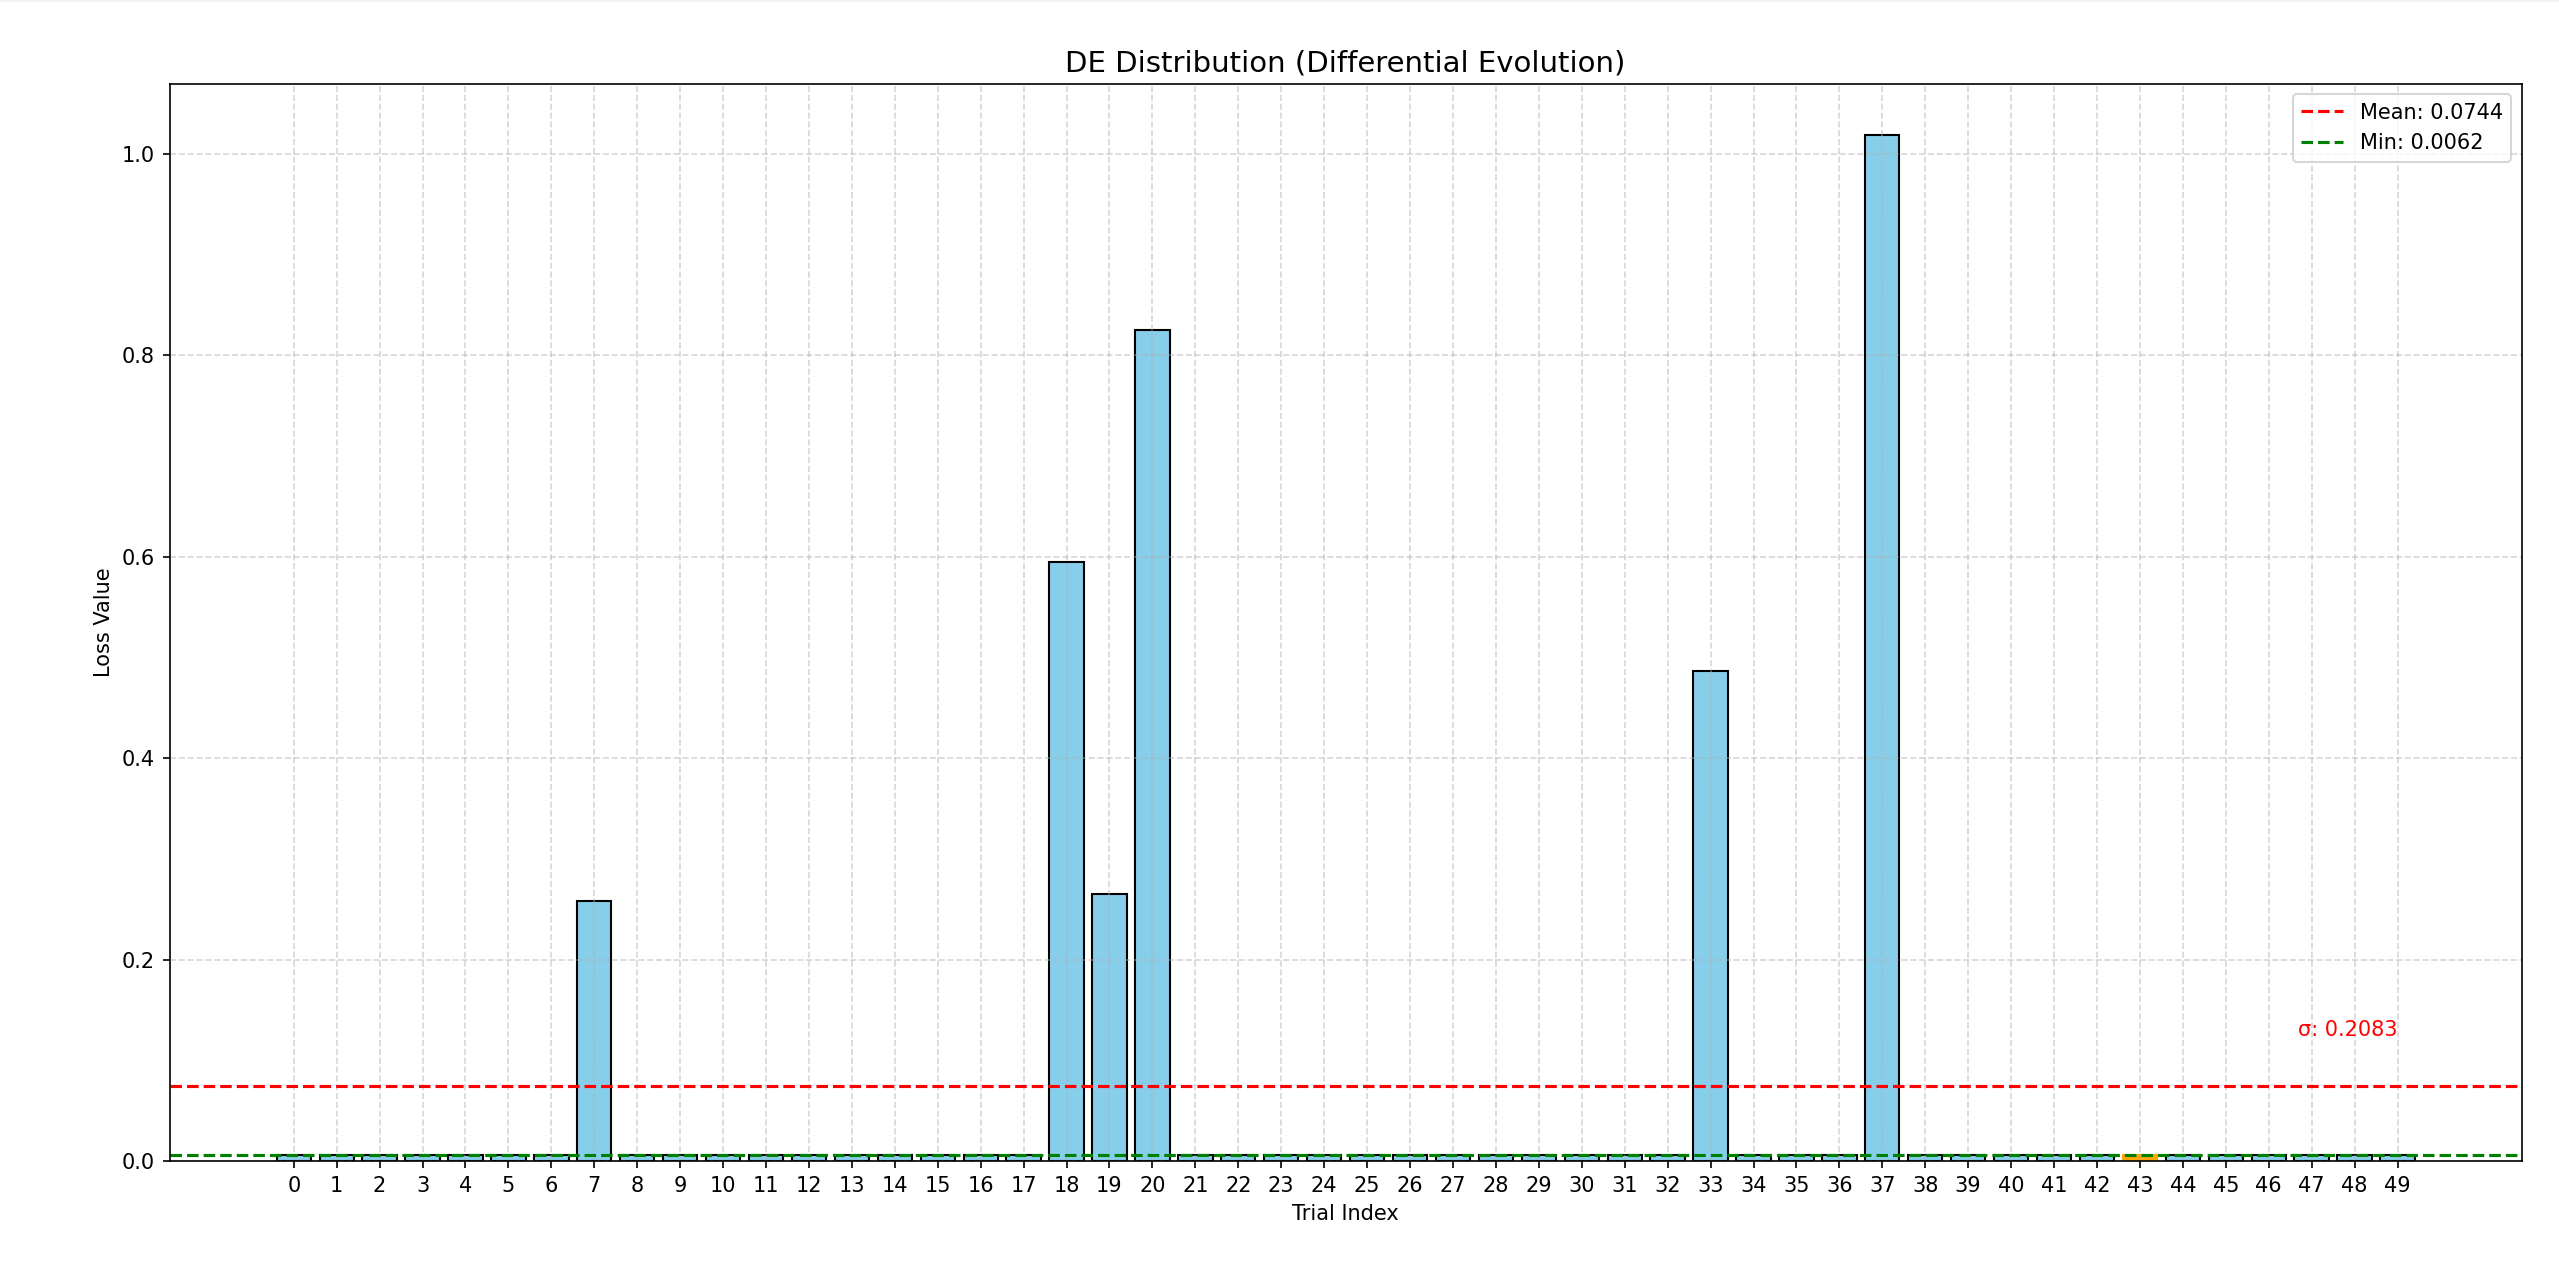
\includegraphics[width=1.0\columnwidth]{figures/DE2000.png}
% \bicaption[50次独立优化实验柱状损失图]{50次独立优化实验柱状损失图。}[Histogram of loss values from 50 independent optimization experiments]{Histogram of loss values from 50 independent optimization experiments.}
% \label{figure3: 柱状loss}
% \end{figure}
% 引用方式:在文字后面加上:\ref{figure3: 柱状loss}

% 表格:
% \begin{table}[h!]
% \small    % 设置表格字体为5号
% \setstretch{1.245}        % 设置具有指定弹力的橡皮长度(原行宽的1.2倍)
% \captionsetup{font={small, stretch=1.512}}
% \centering
%\bicaption[不同基色图像的伽马参数估计结果]{不同基色图像的伽马参数估计结果。}[Gamma parameter estimation results for different primary color images]{Gamma parameter estimation results for different primary color images.}    % 中英文标题


\section[\hspace{-2pt}问题一:路旅游方案设计]{{\heiti\zihao{-3} \hspace{-8pt}问题一:路旅游方案设计}}\label{section3: 问题1:路旅游方案设计}

\subsection[\hspace{-2pt}模型建立与求解]{{\heiti\zihao{4} \hspace{-8pt}模型建立与求解}}\label{section3: 模型建立与求解}

对于此问题,我们首先通过Floyd‑Warshall算法补全邻接矩阵,得到任意两点之间的最短距离。这样我们就可以得到任意区域到任意景点的交通费用和交通时间。此外,我们还需要考虑到旅游信息(住宿、美食、景点等)对方案的影响。既要考虑其对方案满意度的增益,也应当考虑到可容纳人数的限制。\cite{ZNXT201901008}以此为基础,我们进行以下建模:

\textbf{景点收益:}由于缺乏具体景点评分数据,我们假设每个景点具有相近的吸引力价值,即此处不加入游客对景点的偏好因素。$P_{max}$表示某一类型的方案的最大满意度(即总是选择游客喜好程度最高的区域3)。

\begin{equation}
  \begin{aligned}
  \text{Pref}^{(d_{p})}_{max}(type)=\begin{cases}
  9\times 1+2=11, & \text{(1日)}\\
  9\times 3+4=31, & \text{(2日)}\\
  9\times 5+6=51, & \text{(3日)}
  \end{cases}
  \end{aligned}
  \end{equation}

以上方程为景区最大收益函数。为了减少数值对模型计算的影响,我们对三种收益进行归一化处理。

\textbf{区域收益:}套餐$p$涉及到的区域的用餐以及住宿体验。根据题目数据,我们将区域喜好度评分$P_{R_{j}}$作为游客在该区域用餐/住宿获得的满意度。如果套餐跨多日,可能涉及多个不同的区域,则将相应区域的偏好分累计。若在同一天中午和晚上都在同一$R_{j}$区域,则游客在该天对区域$R_{j}$的体验包括午餐和晚餐+住宿,为方便建模并突出问题的重心,我们采用叠加的方式计算区域满意度。

\textbf{交通的时间与费用成本:}每套旅游方案中的交通费用和时间开销会降低满意度。我们采用函数$Cost(p)$来评价一个方案中的所有交通费用,用$Time(p)$来表示所有时间开销。此外我们为其增加了权重$w_{\text{cost}}, w_{\text{time}}$,以此代表不同套餐的倾向,用以区分经济优先还是时间优先。

\begin{equation}
\begin{aligned}
  \text{Cost}(p) = \sum_{(S_i,R_j)\in p}{d(S_i,R_j)}
\end{aligned}
\end{equation}

\begin{equation}
  \begin{aligned}
    \text{Time}(p) = \sum_{(S_i,R_j)\in p}{t(S_i,R_j)}
  \end{aligned}
\end{equation}
  



总的某方案$p$的满意度函数如下:

\begin{equation}
\begin{aligned}
  u_p \;=\; w_{\text{pref}}\frac{\text{Pref}(p)}{\text{Pref}_{\max}^{(d_p)}} \;-\; w_{\text{cost}}\frac{\text{Cost}(p)}{\max\{\text{Cost}(q):q\in \mathcal{P}\}} \;-\; w_{\text{time}}\frac{\text{Time}(p)}{\max\{\text{Time}(q):q\in \mathcal{P}\}},
\end{aligned}
\end{equation}

\textbf{最大化函数:}
\begin{equation}
  \begin{aligned}
    Z = \sum_{p\in \mathcal{P}}u_{p}\cdot x_{p}.
  \end{aligned}
\end{equation}

约束条件如下:

\noindent\textbf{1.景点接待容量限制:}
各景点在各个半天时段的接待总人数不得超限。由于早午两段和最多3天行程共有6个半天时段,模型将假设景点容量可在不同时段重复利用。对每个景点 $i\in S$ 有:

\begin{equation}
  \begin{aligned}
    \sum_{p\in \mathcal{P}}\delta_{i,p}\cdot x_{p} \leq 6\,C_{S_{i}},\quad i=1,2\dots ,6,
  \end{aligned}
\end{equation}
其中$\delta_{i,p}=1$当路线$p$包含景点$i$(即游客在某一时段游览了景点$i$),否则$\delta_{i,p}=0$。

\noindent\textbf{2.午餐餐厅容量约束:}
每个区域的午餐接待能力(每天中午)也限制了路线分配。类似地,如果认为最多3个中午时段可复用,则对每个区域 $j\in R$:

\begin{equation}
  \begin{aligned}
    \sum_{p\in \mathcal{P}}\theta_{j,p}\cdot x_{p} \leq 3\,L_{R_{j}},\quad j=1,2,\dots ,6,
  \end{aligned}
\end{equation}
其中$theta_{j,p}$代表路线$p$在中午曾安排于区域$j$就餐次数(一日游有1次午餐、三日游有3次午餐机会,但可能某些路线会重复去某一区域)。代码中简化为每个区域午餐总游客$\le C^{\text{lunch}}_j$,相当假定所有行程共用一个中午时段容量,这在行程跨多日的情况下略趋保守。

\noindent\textbf{3.晚餐及住宿容量约束:}
每个区域用于晚餐和住宿的容量在不同夜晚也可重复利用。三日游行程最多涉及2晚,故每区域最多2个夜晚可安排住宿。对每个区域 $j\in R$:
\begin{equation}
  \begin{aligned}
    \sum_{p\in \mathcal{P}}\phi_{j,p}\cdot x_p \;\le\; 2\,C^{\text{night}}_j, \quad j=1,\dots,6,
  \end{aligned}
\end{equation}

其中$\phi_{j,p}$为路线$p$在夜晚留宿于区域$j$的次数(二日游路线有1晚、三日游有2晚,一般假定同一线路不重复入住同一酒店区域)。

\noindent\textbf{4.游客总数约束:}
根据预期需求,分别规定各类行程分配的总游客数。例如,设定选择一日游的游客总数为$N_{1}$人、二日游$N_{2}$人、三日游$N_{3}$人。则对每一种行程类型分别有:
\begin{equation}
  \begin{aligned}
    \sum_{p\in P_{1\text{day}}}x_p = N_{1},\qquad \sum_{p\in P_{2\text{day}}}x_p = N_{2},\qquad \sum_{p\in P_{3\text{day}}}x_p = N_{3}.    
  \end{aligned}
\end{equation}

代码实现中分别令一日游、二日游总游客数为30,000,三日游为20,000。

约束处理完成后,我们将采用枚举的方式得到一日游、二日游等的所有可能方案。再将其加入到MILP模型中。结合遗传算法选择高质量路线,并采用启发式规则进行路线多样化拓展。最终得到最合适的旅游路线。

\subsection[\hspace{-2pt}问题一结果分析]{{\heiti\zihao{4} \hspace{-8pt}问题一结果分析}}\label{section4: 问题一结果分析}

根据$w_{cost}$和$w_{time}$的不同权重配置,我们可以设置不同权重,得到不同侧重点的旅游方案。本论文设置了三种情况,并对优化结果进行了详细分析。

\textbf{均衡型(费用权重=0.5,时间权重=0.5):}

均衡型配置追求费用和时间的平衡优化。实验结果显示:一日游方案成功分配3万游客到2条最优路线,平均满意度达到0.47;二日游方案分配3万游客到4条路线,总费用302.7万元,总时间5541万分钟,平均满意度0.39;三日游方案分配2万游客到4条路线,总费用355.06万元,平均满意度0.34。该配置在各项指标间取得了良好的平衡,适合大多数游客的需求。

\textbf{费用优先型(费用权重=0.7,时间权重=0.3):}

费用优先型配置更注重控制旅游成本。对比分析发现:在一日游方案中,费用优先型与均衡型结果完全一致,说明一日游路线已达到成本最优;二日游方案中,总费用降低至292.92万元,相比均衡型节省了9.78万元(降幅3.2%),但时间成本略有增加至5745万分钟;三日游方案表现最为突出,总费用大幅降低至341.32万元,相比均衡型节省13.74万元(降幅3.9%),同时平均满意度还提升至0.36。这表明费用优先型配置能够有效控制成本,特别适合预算敏感的游客群体。

\textbf{时间优先型(费用权重=0.3,时间权重=0.7):}

时间优先型配置侧重于减少旅行时间。结果显示:一日游和二日游方案与均衡型完全相同,表明在这两种方案中时间已达到最优配置;三日游方案中,虽然总费用略有增加至367.6万元,但时间安排更为紧凑高效。值得注意的是,时间优先型在路线选择上呈现出不同的偏好模式,优先选择时间效率更高的景点组合和区域路径,适合时间有限但希望充分体验的游客。

\textbf{综合比较分析:}

通过三种配置的对比分析可以发现:(1)一日游方案在三种配置下结果一致,说明短期旅游路线的优化空间有限,已达到全局最优;(2)二日游方案中费用优先型在成本控制方面具有明显优势,适合预算约束较强的情况;(3)三日游方案显示出最大的优化弹性,不同权重配置产生显著差异,为不同需求的游客提供了多样化选择;(4)所有配置均成功实现了大规模游客分流,验证了模型的实用性和有效性。这些结果为旅游管理部门制定差异化的旅游产品策略提供了科学依据。



\section[\hspace{-2pt}问题二:方案优化]{{\heiti\zihao{-3} \hspace{-8pt}问题二:方案优化}}\label{section3: 问题2:方案优化}

\subsection[\hspace{-2pt}问题分析与建模目标]{{\heiti\zihao{4} \hspace{-8pt}问题分析与建模目标}}\label{section2: 问题分析与建模目标}

根据问题分析,我们设计了如下的距离函数,综合考虑了方案间的景点、路线、区域等相似度,将重复性较强的方案合并。由于景点和区域皆为符号度量,因此二者都采用了Jaccard相似度。类型相似度用以判断旅游天数是否相同,可以保证同一聚类中心皆为同一天数。余下的偏好相似度、成本相似度和时间相似度都采用了欧氏距离,成本相似度采用了欧氏距离,时间相似度采用了欧氏距离。

\noindent\textbf{1.景点相似度:}
\begin{equation}
  \begin{aligned}
    \text{Simu}_{p_{i},p_{j},S} = \frac{|\underset{S\in p_i}{\bigcup}\cap \underset{S\in p_j}{\bigcup}|}{|\underset{S\in p_i}{\bigcup}\cup \underset{S\in p_j}{\bigcup}|}
  \end{aligned}
\end{equation}

\noindent\textbf{2.类型相似度:}
\begin{equation}
  \begin{aligned}
    \text{Simu}_{p_{i},p_{j},Day} = \begin{cases}
      1, & \text{若}d_{p_i}=d_{p_j}\\
      0, & \text{否则}
    \end{cases}
  \end{aligned}
\end{equation}

\noindent\textbf{3.区域相似度:}
\begin{equation}
  \begin{aligned}
    \text{Simu}_{p_{i},p_{j},R} = \frac{|\underset{R\in p_i}{\bigcup}\cap \underset{R\in p_j}{\bigcup}|}{|\underset{R\in p_i}{\bigcup}\cup \underset{R\in p_j}{\bigcup}|}
  \end{aligned}
\end{equation}

\noindent\textbf{4.偏好相似度:}
\begin{equation}
  \begin{aligned}
    \text{Simu}_{p_{i},p_{j},P} = 1-\frac{|\text{Pref}(p_{i})-\text{Pref}(p_{j})|}{\text{max}(\text{Pref}(p_{i}),\text{Pref}(p_{j}))}
  \end{aligned}
\end{equation}

\noindent\textbf{5.成本相似度:}
\begin{equation}
  \begin{aligned}
    \text{Simu}_{p_{i},p_{j},C} = 1-\frac{|\text{Cost}(p_{i})-\text{Cost}(p_{j})|}{\text{max}(\text{Cost}(p_{i}),\text{Cost}(p_{j}))}
  \end{aligned}
\end{equation}

\noindent\textbf{6.时间相似度:}
\begin{equation}
  \begin{aligned}
    \text{Simu}_{p_{i},p_{j},T} = 1-\frac{|\text{Time}(p_{i})-\text{Time}(p_{j})|}{\text{max}(\text{Time}(p_{i}),\text{Time}(p_{j}))}
  \end{aligned}
\end{equation}

定义好以上相似度后,就可以计算两个方案之间的加权距离。

\begin{equation}
  \begin{aligned}
    D(p_{i},p_{j}) = \sum_{k\in \text{Temp}}^{6}w_{k}\cdot\text{Simu}_{p_{i},p_{j},k},\quad \text{Temp}=\{S,Day,R,P,C,T\}
  \end{aligned}
\end{equation}

以上因素综合考虑到不同旅行方案在景点、区域、偏好等多个方面的相似度,可以得到不同旅行方案之间的距离。在完成“旅游方案相似度”加权距离函数的数学建模后,下一步便可对所有候选路线实施 K‑means 聚类。

% 基于旅游方案相似度的加权距离函数建模完成后,即可进行K均值聚类。算法会尝试不同的K值,并根据簇内平方和选择最优的K值作为最终的结果。

% 当要求旅游套餐种类总数不超过10种时,需要对上述模型进行适应性修改。原模型在追求最大满意度下,可能启用许多不同路线方案来绕开局部容量瓶颈,从而方案种类较多。如果限制套餐类型数$\le10$,模型必须在满意度与管理简化之间折中。我们做出了如下调整:

% \noindent\textbf{加入套餐数量约束:}增加约束$\displaystyle\sum_{p\in P} \le 10$,限制被选用的不同路线方案数不超过10种。其中为0-1变量,表示方案$p$是否被采用。并引入逻辑约束$x_p \le N_{\text{total}};$(或大$M$法)将$x_p$与关联。这样仅当$y=1$时,$x_p$可取正值,否则该路线不分配游客。此调整实质上将线性规划扩展为混合整数规划,有助于直接在求解过程中控制方案种类数上限。

% \noindent\textbf{精选候选路线集:}在模型求解前预先筛选和精简路线集合$P$,只保留若干“优选”套餐候选。比如,根据单条路线的满意度系数$u_p$对候选方案排序,选取满意度高且覆盖面广的前若干条路线进入优化。原模型生成的路线非常多(一日游$6\times5\times6=180$种,二日游上限$10^4$种,三日游经遗传算法+启发式生成5000种),有许多方案实际贡献的游客数很小甚至为0。我们可剔除明显次优或冗余的方案,例如去除行程过长费用偏高而偏好分较低的组合,或者对行程相似且收益接近的方案只保留其中一种。这相当于在不增加过多成本的前提下人工设定候选集精简至$\le10$条路线,然后在此基础上重新优化分配。这种路线筛选(如按满意度排序取Top 10)和聚类归并的方法可极大减少方案种类,同时尽量保证总满意度接近原最优值。

% \noindent\textbf{优先级调度与容量放宽:}在仅允许提供有限几种套餐时,可考虑适当调整对容量约束的处理,确保主要景点和区域得到利用。例如,将重点偏好的景点设计为\**固定线路**,优先占用一定游客量,然后对剩余游客采用次优线路。在代码实现层面,可以对生成的候选路线按照偏好得分或单位满意度收益排序,优先选取少数几条高效路线分配游客直到触及某一容量约束,再引入下一优方案。这种贪心分配过程可以模拟人工规划几种典型套餐的思路:例如优先设计几条涵盖热门景区且总体花费合理的线路,再视剩余接待资源补充其他路线,从而将总套餐数控制在上限之内。

% 综上,当限制套餐总数不超过10种时,模型需要从“穷尽所有可能组合求全局最优”转变为“在有限方案中求近优”。这要求在模型中增加**组合选择的决策变量和约束**,或采用启发式策略筛选方案。通过上述调整,既能满足管理方便的要求,又尽可能兼顾游客满意度和资源利用的均衡。模型的结构与求解思路具有一定灵活性:无论是通过加入$y$变量实现严格的种类约束,还是通过缩减候选路线集来隐含满足要求,都体现了对原优化模型的适应性改进。

\subsection[\hspace{-2pt}模型求解和结果分析]{{\heiti\zihao{4} \hspace{-8pt}模型求解和结果分析}}\label{section2: 模型求解和结果分析}

具体流程如下:首先,以距离函数 $D(\cdot,\cdot)$ 为度量,对给定的 K 值(簇数)运行多次随机初始化的 K‑means++,获得每个 k 下的最小 簇内平方和。随后,将 k 在预设范围 $3,\dots ,6$ 内逐一取值。最终选择使指标综合最优的 $K$。确定 $K$ 后,以其为簇数重新运行 K‑means,并选取每个簇中净收益最高或代表性最强的方案,形成至多 10 种、覆盖多样化场景且经济效益最优的扩容套餐。

% 以下是K-means聚类算法流程:
\begin{algorithm}[H]\small
  \setstretch{1.245}
  \renewcommand{\algorithmcfname}{算法}
  \caption{旅游路线相似度聚类算法}\label{alg:kmeans_route}

  \KwIn{可行路线集合 $\mathcal R$(已转为特征向量);候选聚类数 $\mathcal K=\{2,3,4,5,6\}$}
  \KwOut{最优聚类数 $k^*$、最终模型 $\mathcal M^*$ 及聚类统计 $\mathcal C$}

  \textbf{步骤1:初始化}\;
  $k^* \leftarrow \text{first}(\mathcal K)$;\;
  $\text{bestInertia}\leftarrow+\infty$\;

  \textbf{步骤2:遍历候选聚类数}\;
  \ForEach{$k\in\mathcal K$}{
      $\mathcal M \leftarrow \texttt{KMeans.fit}(\mathcal R,k)$\;
      \If{$\mathcal M.\texttt{inertia\_}<\text{bestInertia}$}{
          $\text{bestInertia}\leftarrow\mathcal M.\texttt{inertia\_}$\;
          $k^*\leftarrow k$\;
      }
  }

  \textbf{步骤3:终极聚类与统计}\;
  $\mathcal M^* \leftarrow \texttt{KMeans.fit}(\mathcal R,k^*)$\;
  $\mathcal C \leftarrow \texttt{GetClusterInfo}(\mathcal M^*,\mathcal R)$\;

  \textbf{步骤4:输出结果}\;
  \Return $(k^*,\mathcal M^*,\mathcal C)$\;
\end{algorithm}

通过K均值算法,我们得到了最优聚类数为6,其中每个簇中净收益最高的方案只保留一种,最终得到了6种旅游方案。以下是方案的详细信息:

\begin{table}[H]\small
  \centering
  \caption{K\,means 聚类结果汇总($k=6$,路线总数 11,惯性值 1.178)}
  \begin{tabularx}{\textwidth}{>{\centering\arraybackslash}m{0.6cm}
                                  >{\centering\arraybackslash}m{1cm}
                                  >{\centering\arraybackslash}m{1cm}
                                  >{\centering\arraybackslash}m{1cm}
                                  >{\centering\arraybackslash}m{1cm}
                                  X
                                  X}
    \toprule
    \textbf{簇} & \textbf{成本/元} & \textbf{时间/分钟} & \textbf{满意度} & \textbf{路线类型} & \textbf{景点路线} & \textbf{区域路线} \\
    \midrule
    0 & 82.0  & 165.0 & 0.392 & 2 day & S1,S4,S6,S2 & R1,R4,R2 \\
    1 & 116.0 & 225.0 & 0.361 & 2 day & S1,S2,S6,S4 & R2,R2,R4 \\
    2 & 25.0  & 45.0  & 0.506 & 1 day & S3,S6 & R3 \\
    3 & 161.0 & 285.00 & 0.401 & 3 day & S1,S4,S6,S5,S3,S2 & R1,R2,R3,R3,R2 \\
    4 & 208.00 & 370.00 & 0.3560 & 3 day & S2,S3,S5,S4,S1,S6 & R2,R3,R4,R4,R2 \\
    5 & 219.00 & 380.00 & 0.348 & 3 day & S3,S6,S5,S2,S4,S1 & R2,R3,R4,R2,R4 \\
    \bottomrule
  \end{tabularx}
  \label{tab:kmeans_summary}
\end{table}



\begin{figure}[h]
\centering
\captionsetup{font={small, stretch=1.312}}
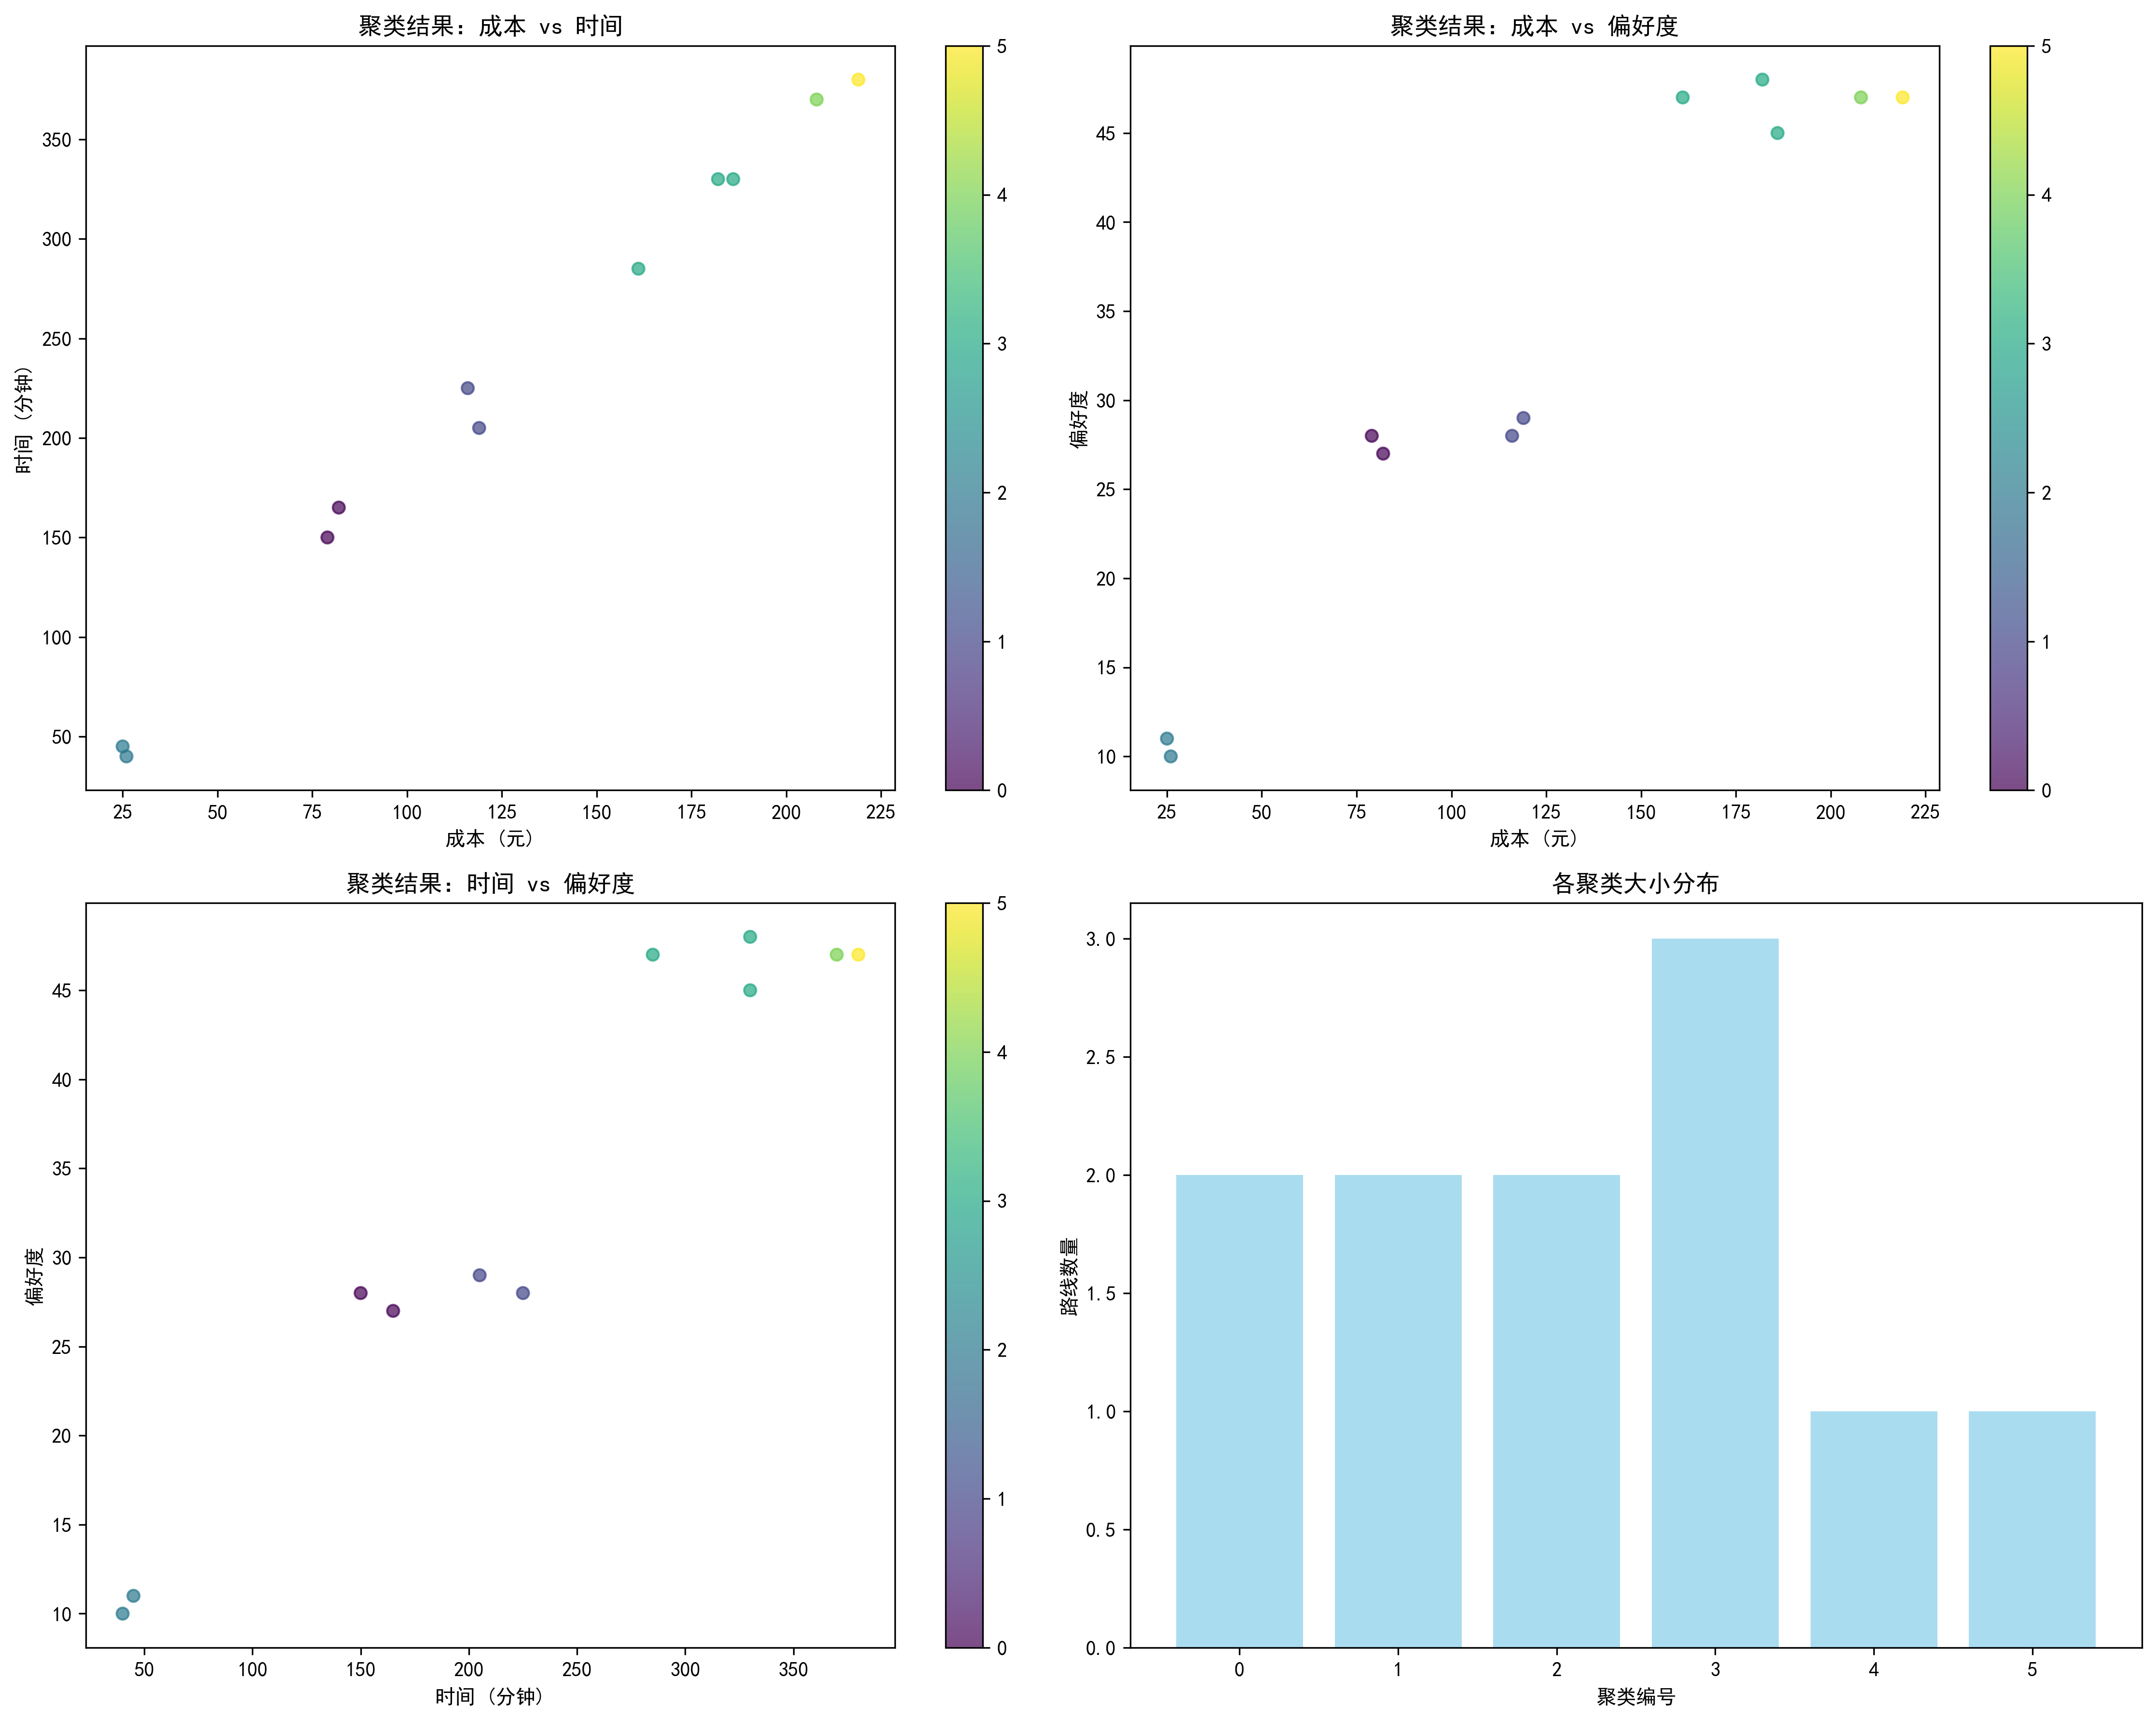
\includegraphics[width=1.0\columnwidth]{figures/tourism_optimization_clusters.png}
\bicaption[聚类结果可视化]{聚类结果可视化图。}[clusterResult]{Histogram of clusterReseult.}
\label{figure3: cluster}
\end{figure}


由以上图表可以看出,聚类结果能够有效地将不同类型的旅游路线进行区分,每个簇代表了具有代表性的出行偏好和路线组合。各方案在成本、时间和满意度等方面表现均衡,能够满足不同游客的需求。整体来看,模型聚类效果良好,结果具有较强的实际参考价值。






\section[\hspace{-2pt}问题三:旅馆建设规模与位置选择]{{\heiti\zihao{-3} \hspace{-8pt}问题三:旅馆建设规模与位置选择}}\label{section4: 问题3:旅馆建设规模与位置选择}

\subsection[\hspace{-2pt}模型建立流程]{{\heiti\zihao{4}\hspace{-8pt}模型建立流程}}\label{subsec:3-model-build}


本模型旨在分析重庆旅游景区的住宿扩容问题,基于游客需求、交通成本、时间消耗和景区容量等因素,通过构建优化模型对扩容方案进行评估。

\noindent\textbf{首先,模型采用了基于规模报酬递减的扩容成本函数:}
\begin{equation}
  \begin{aligned}
    C(\Delta K)=c_{1}(\Delta K)^{\gamma}, \quad c_{1} =7\times 10^{-4}\text{(亿元)}, \gamma = 1.09
  \end{aligned}
\end{equation}

此扩容成本函数是采用来自网络的数据统计,并进行处理后得到的。

\noindent\textbf{并定义了经济收益函数 $B(\Delta K)$:}

\begin{equation}
  \begin{aligned}
    B(\Delta K) = v_{s}[Z(K)-Z(K^0)]+v_{p}[N(K)-N(K^{0})]
  \end{aligned}
\end{equation}

其中考虑了扩容后满意度增量和游客接待量的增量。满意度增量通过扩容后游客对旅游线路的偏好变化进行计算,接待量增量则基于实际可接待游客人数与扩容前的差异。

\noindent\textbf{扩容决策的目标是最大化净收益:}

\begin{equation}
  \begin{aligned}
    \underset{r,\Delta K\geq 0}{max}  F_r(\Delta K) = B_r(\Delta K) - C(\Delta K)
  \end{aligned}
\end{equation}

即通过选择最优区域和扩容规模 $\Delta K$,使得总的经济效益最大。模型通过枚举不同区域和容量增量,计算每种方案的经济收益,并结合遗传算法和线性规划(MILP)对扩容后的最优游客分配进行求解。最终,选出净收益最大的扩容方案,并提供详细的扩容规模及其对应的效益曲线。



该模型不仅帮助政府和企业做出最优的扩容决策,还能评估不同扩容方案的经济影响,为旅游业的长期规划提供支持。

\subsection[\hspace{-2pt}模型求解]{{\heiti\zihao{4}\hspace{-8pt}模型求解}}\label{subsec:3-model-build}

模型的求解采用“双层结构”。外层离散搜索扩容区域$r$与规模$\Delta K$,内层维持既有的“枚举路线结合MILP”的流程:

\noindent\textbf{外层:}

\begin{equation}
  \begin{aligned}
    \underset{r,\Delta K \geq 0}{max} F_{r}(\Delta K)
  \end{aligned}
\end{equation}

\noindent\textbf{内层:}
\begin{equation}
  \begin{aligned}
    Z(K),N(K)=arg\quad \underset{x}{max} \sum_{i}s_{i}x_{i}\\
    s.t. \text{容量约束}K
  \end{aligned}
\end{equation}

具体算法如下所示:

\begin{algorithm}[H]\small
  \setstretch{1.245}
  \renewcommand{\algorithmcfname}{算法}
  \caption{旅游景区扩容优化算法}

  \KwIn{原始夜宿容量 $K_0=(K_1^0,\dots,K_6^0)$;扩容步长集合
        $\Delta\mathcal K=\{0,0.5,1,\dots,\Delta K_{\max}\}$;游客需求 $T^0$}
  \KwOut{最优扩容区域 $r^*$、规模 $\Delta K^*$ 及最大净收益 $F^*$}

  \textbf{步骤1:基准求解}\;
  $\text{base\_results}\leftarrow\text{optimizer.run\_optimization}(K_0)$\;
  取 $Z(K^0),\,N(K^0)$\;

  \textbf{步骤2:区域与扩容规模枚举}\;
  \For{$r\leftarrow1$ \KwTo $6$}{
    \For{${\Delta K}\in\Delta\mathcal K$}{
      $K_r \leftarrow K_r^0 + \Delta K$\tcp*{修改容量上限}
      $\text{cur} \leftarrow \text{optimizer.run\_optimization}(K_r)$\;
      取 $Z(K),\,N(K)$\;
      $B = v_s\bigl[Z(K)-Z(K^0)\bigr] + v_p\bigl[N(K)-N(K^0)\bigr]$\;
      $C = 0.0007\,(\Delta K)^{1.09}$\;
      $F(r,\Delta K) = B - C$\;
    }
  }

  \textbf{步骤3:选择最优方案}\;
  $(r^*,\Delta K^*) = \arg\max_{r,\Delta K} F(r,\Delta K)$\;
  $F^* \leftarrow F(r^*,\Delta K^*)$\;

  \textbf{步骤4:绘制净收益曲线}\;
  绘制 $F(r,\Delta K)$ 随 $\Delta K$ 变化的曲线,并标注 $(r^*,\Delta K^*)$\;

  \label{algorithm:expansion_optimization}
\end{algorithm}

\subsection[\hspace{-2pt}结果分析]{{\heiti\zihao{4}\hspace{-8pt}结果分析}}\label{subsec:3-model-build}
在完成模型求解后,净收益曲线清晰展示了不同区域在不同扩容规模下的经济效益。下表汇总了主要扩容方案的关键指标,并按净收益从高到低排序。并且为进一步直观对比扩容规模与净收益关系,绘制了不同区域在多种扩容方案下的净收益分布。以下是得出的结论:
\begin{enumerate}
  \item \textbf{区域3呈现显著经济优势}:前七大高收益方案均集中于区域3,其中以扩容 1.00~万人次的方案最优,净收益达 74.32~亿元,其次为 2.00~万人次(70.43~亿元)与 1.50~万人次(57.90~亿元)。
  \item \textbf{净收益对扩容规模并非单调增加}:区域3扩容从 1.00 提升至 2.00~万人次时,净收益下降,体现边际效益递减。曲线走势亦证实存在一最佳扩容规模区间。
  \item \textbf{其他区域仍具备潜力}:区域4 在小规模扩容(0.50~万人次)下即可带来 33.19~亿元收益;区域5 与区域1 的部分方案亦具备可观回报,但整体低于区域3;区域2 受限于基础容量与偏好,收益相对有限。
\end{enumerate}

\begin{table}[htbp]\small
  \centering
  \caption{旅馆扩容方案净收益分析结果}
  \label{tab:expansion-results}
  \begin{tabularx}{\textwidth}{c c c c c}
    \toprule
    \textbf{区域} & \textbf{扩容规模/万人次} & \textbf{原容量/万人次} & \textbf{新容量/万人次} & \textbf{净收益/亿元} \\
    \midrule
    区域3 & 1.00 & 0.66 & 1.66 & 74.3205 \\
    区域3 & 2.00 & 0.66 & 2.66 & 70.4321 \\
    区域3 & 1.50 & 0.66 & 2.16 & 57.9014 \\
    区域3 & 4.50 & 0.66 & 5.16 & 53.2195 \\
    区域3 & 3.00 & 0.66 & 3.66 & 48.7040 \\
    区域3 & 4.00 & 0.66 & 4.66 & 46.9166 \\
    区域3 & 5.00 & 0.66 & 5.66 & 44.5128 \\
    区域4 & 0.50 & 2.16 & 2.66 & 33.1853 \\
    区域3 & 0.50 & 0.66 & 1.16 & 30.0672 \\
    区域3 & 3.50 & 0.66 & 4.16 & 29.9084 \\
    区域5 & 4.00 & 1.38 & 5.38 & 28.5287 \\
    区域5 & 3.50 & 1.38 & 4.88 & 28.0013 \\
    区域1 & 1.00 & 1.14 & 2.14 & 27.6119 \\
    区域5 & 2.00 & 1.38 & 3.38 & 25.1312 \\
    区域3 & 2.50 & 0.66 & 3.16 & 24.3754 \\
    区域2 & 1.00 & 1.92 & 2.92 & 24.1800 \\
    区域1 & 1.50 & 1.14 & 2.64 & 23.6578 \\
    区域5 & 0.00 & 1.38 & 1.38 & 23.5974 \\
    区域1 & 2.00 & 1.14 & 3.14 & 22.2397 \\
    区域1 & 0.00 & 1.14 & 1.14 & 20.2017 \\
    \bottomrule
  \end{tabularx}
\end{table}
\begin{figure}[htbp]
  \centering
  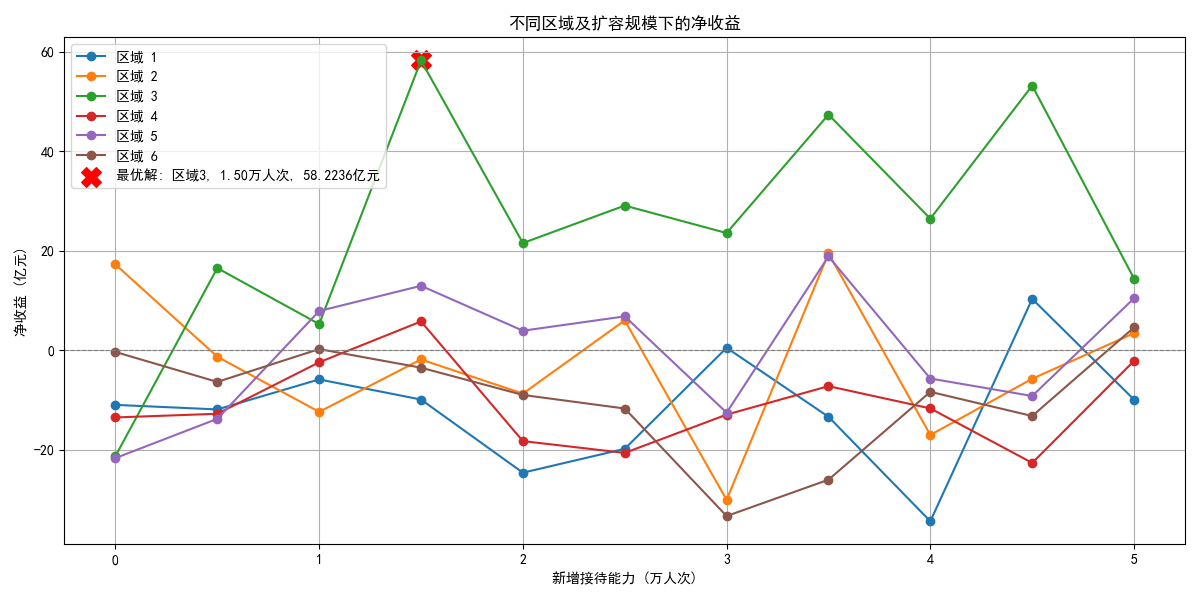
\includegraphics[width=0.8\textwidth]{figures/net_benefit_vs_expansion.png}
  \caption{不同区域扩容规模与净收益关系图}
  \label{fig:net-benefit-expansion}
\end{figure}




%\chapter[\hspace{0pt}模型实现与结果分析]{{\heiti\zihao{3}\hspace{0pt}模型实现与结果分析}}\label{chapter4: 模型实现与结果分析}
\removelofgap
\removelotgap

\section[\hspace{-2pt}数据集介绍]{{\heiti\zihao{-3} \hspace{-8pt}数据集介绍}}\label{section4: 数据集介绍}

\section[\hspace{-2pt}实验设计]{{\heiti\zihao{-3} \hspace{-8pt}实验设计}}\label{section4: 实验设计}

\section[\hspace{-2pt}结果与分析]{{\heiti\zihao{-3} \hspace{-8pt}结果与分析}}\label{section4: 结果与分析}


%\chapter[\hspace{0pt}模型评价]{{\heiti\zihao{3}\hspace{0pt}模型评价}}\label{chapter4: 模型评价}
\removelofgap
\removelotgap

\section[\hspace{-2pt}数据集介绍]{{\heiti\zihao{-3} \hspace{-8pt}数据集介绍}}\label{section4: 数据集介绍}

\section[\hspace{-2pt}实验设计]{{\heiti\zihao{-3} \hspace{-8pt}实验设计}}\label{section4: 实验设计}

\section[\hspace{-2pt}结果与分析]{{\heiti\zihao{-3} \hspace{-8pt}结果与分析}}\label{section4: 结果与分析}

\chapter[\hspace{0pt}模型评价与推广]{{\heiti\zihao{3}\hspace{0pt}模型评价与推广}}\label{chapter4: 模型评价与推广}
\removelofgap
\removelotgap

\section[\hspace{-2pt}主要结论]{{\heiti\zihao{-3} \hspace{-8pt}主要结论}}\label{section5: 主要结论}

通过构建基于混合整数线性规划的多目标优化模型,成功实现了重庆旅游路线的智能分配,主要取得以下成果:

\noindent\textbf{多目标优化效果显著}:基于费用、时间和满意度的多目标优化模型能够有效平衡各项指标。实验结果表明,不同权重配置下的优化方案都能适应不同游客需求,其中费用优先型配置在三日游方案中表现最优,总费用降低至341.32万元,平均满意度提升至0.36。

\noindent\textbf{算法融合策略有效}:采用Floyd-Warshall算法预处理交通矩阵,结合遗传算法和启发式方法生成候选路线,最终通过混合整数线性规划求解最优分配。混合方法成功生成1200+条高质量候选路线,证明了多算法融合策略在大规模优化问题中的有效性。

\section[\hspace{-2pt}模型优点]{{\heiti\zihao{-3} \hspace{-8pt}模型优点}}\label{section5: 模型优点}

\subsection[\hspace{-2pt}问题一模型优点]{{\heiti\zihao{4} \hspace{-8pt}问题一模型优点}}\label{subsection5: 问题一模型优点}

\noindent\textbf{多重实际约束考虑}:模型通过引入土壤轮作、作物销售限制、耕地面积限制等多项约束,确保了种植计划的可行性和合理性。在理论上,这种方法符合农业生产中的多重约束条件,能够反映现实中的复杂限制,确保每个决策变量的有效性。

\noindent\textbf{MILP求解方法优势}:MILP方法在理论和计算上具有良好的解决能力,尤其适合处理复杂的多维决策问题。通过采用该方法,可以在保证模型准确性的同时,迅速找到全局最优解,具有较强的计算效率和扩展性。
\subsection[\hspace{-2pt}问题二模型优点]{{\heiti\zihao{4} \hspace{-8pt}问题二模型优点}}\label{subsection5: 问题二模型优点}

\noindent\textbf{考虑不确定性}:通过引入蒙特卡洛采样(SAA)方法,模型能够有效地处理市场需求、单产、价格波动和种植成本的随机性。这使得模型能够更准确地反映未来农业生产中的不确定性,从而提供更为稳健的种植方案。

\noindent\textbf{优化收益和风险}:模型通过引入风险系数 $\lambda$,使得优化目标不仅仅是追求最大化的收益,还兼顾了风险管理。通过最小化收益的波动(方差),模型能够在收益和风险之间找到平衡,适应不同的风险偏好。

\noindent\textbf{灵活性强}:模型能够根据不同的场景生成需求、单产、价格和成本的随机增量,使得可以对不同的市场或环境变化进行适应性分析。用户可以根据需要选择不同的场景数量以及风险偏好,调整优化结果。

\subsection[\hspace{-2pt}问题三模型优点]{{\heiti\zihao{4} \hspace{-8pt}问题三模型优点}}\label{subsection5: 问题三模型优点}

\noindent\textbf{替代性与互补性考虑}:本模型在作物种植优化过程中引入了作物之间的替代性和互补性理论。这种替代性和互补性假设在农业经济学中有着广泛的应用,能够反映不同作物间的市场联动效应,提高了模型的经济性和准确性。
\noindent\textbf{轮作与增产效应线性化}:轮作和互补增产效应通过Big-M方法进行线性化处理,使得本模型依然能够通过MILP方法求解。该理论方法在保持模型计算可行性的同时,能够准确反映农业生产中的增产效应和土壤改良效应,提高了模型的现实适应性。
\noindent\textbf{价格与需求精细调整}:模型通过调整价格系数和有效需求关系,精确模拟了作物间的市场联动效应。在理论上,这种方法能够准确反映价格波动对作物销售的影响,并使得优化方案更符合市场实际需求。
\section[\hspace{-2pt}不足与改进方向]{{\heiti\zihao{-3} \hspace{-8pt}不足与改进方向}}\label{section5: 不足与改进方向}

\subsection[\hspace{-2pt}问题一模型的主要局限]{{\heiti\zihao{4} \hspace{-8pt}问题一模型的主要局限}}\label{subsection5: 问题一模型局限}

\noindent\textbf{不考虑市场需求波动}: 销售量和价格假设稳定,未考虑到市场供需变化对收益的影响。
\subsection[\hspace{-2pt}问题一模型的改进方向]{{\heiti\zihao{4} \hspace{-8pt}问题一模型的改进方向}}\label{subsection5: 问题一模型改进}
增加市场需求变化和价格波动的动态因素,模拟市场不确定性,改进预期销售量和单价的估计。
\subsection[\hspace{-2pt}问题二模型的主要局限]{{\heiti\zihao{4} \hspace{-8pt}问题二模型的主要局限}}\label{subsection5: 问题二模型局限}


\noindent\textbf{计算复杂度较高}:随机模拟和多场景求解增加了模型的计算复杂度,尤其是在考虑多个场景的情况下,求解过程可能会变得非常耗时。

\subsection[\hspace{-2pt}问题二模型的改进方向]{{\heiti\zihao{4} \hspace{-8pt}问题二模型的改进方向}}\label{subsection5: 问题二模型改进}


\noindent\textbf{优化计算方法}:可以采用启发式算法或近似算法(如遗传算法或模拟退火算法)来降低计算复杂度,同时保证模型的求解效率。


\subsection[\hspace{-2pt}问题三模型的主要局限]{{\heiti\zihao{4} \hspace{-8pt}问题三模型的主要局限}}\label{subsection5: 问题三模型局限}


\noindent\textbf{轮作增益的估算不准确}:轮作增益系数假设较为简单,可能忽略了一些农业生态因素的复杂性,导致增益估算存在误差。

\subsection[\hspace{-2pt}问题三模型的改进方向]{{\heiti\zihao{4} \hspace{-8pt}问题三模型的改进方向}}\label{subsection5: 问题三模型改进}


\noindent\textbf{加强数据校准与灵敏度分析}:加强市场数据和模型假设的校准,并进行灵敏度分析,评估模型对参数变化的敏感性,提高模型的稳健性和可信度。



%\include{contents/yourFreeChoise}

\backmatter %%% 后置部分(致谢、参考文献、附录等)

%% 参考文献
% 顺序编码制:cqunumerical		
% 注意:至少需要引用一篇参考文献,否则下面两行会引起编译错误。
% \bibliographystyle{cqunumerical}
\bibliographystyle{gbt7714-numerical_new}
\bibliography{ref/refs}


%% 附录(按ABC...分节,证明、推导、程序、个人简历等)
\appendix
\chapter[附\hskip\ccwd{}\hskip\ccwd{}录]{{\heiti\zihao{3}附\hskip\ccwd{}\hskip\ccwd{}录}}

\section[\hspace{-2pt}支撑材料总览]{{\heiti\zihao{-3} \hspace{-8pt}支撑材料总览}}

% 本论文的所有支撑材料组织在\texttt{MathModel\_Code/}目录下,
具体分类和说明如表\ref{table:supporting_materials}所示:

\begin{table}[h!]
\footnotesize
\setstretch{1.1}
\captionsetup{font={small, stretch=1.512}}
\centering
\bicaption[支撑材料分类说明]{支撑材料分类说明。}[Classification of Supporting Materials]{Classification of Supporting Materials.}
\begin{tabularx}{\textwidth}{p{1.8cm}p{4.2cm}X}
\toprule
材料类型 & 文件路径 & 说明 \\
\midrule
\multirow{3}{1.8cm}{实现代码} & \texttt{B/p1/p1.py} & 问题1:BT.2020到sRGB色域映射优化 \\
 & \texttt{B/p2/p2.py} & 问题2:四通道到五通道神经网络转换 \\
 & \texttt{B/p3/p3.py} & 问题3:LED显示器颜色校正算法 \\
\midrule
\multirow{4}{1.8cm}{原始数据} & \texttt{data/origin/xlsx/B题附件:RGB数值.xlsx} & 题目提供的原始RGB数值 \\
 & \texttt{data/preprocess/}\newline\texttt{RedPicture.xlsx} & 预处理后的红色基图数据 \\
 & \texttt{data/preprocess/}\newline\texttt{GreenPicture.xlsx} & 预处理后的绿色基图数据 \\
 & \texttt{data/preprocess/}\newline\texttt{BluePicture.xlsx} & 预处理后的蓝色基图数据 \\
\midrule
\multirow{9}{1.8cm}{结果图像} & \texttt{results/p1/DE2000.png} & 问题1:50次优化$\Delta E_{00}$分布 \\
 & \texttt{results/p1/色度.png} & 问题1:CIE1931色度图对比 \\
 & \texttt{results/p1/面积Loss.png} & 问题1:色域面积差异分析 \\
 & \texttt{results/p2/}\newline\texttt{Training\_Loss\_Curve.png} & 问题2:神经网络训练损失曲线 \\
 & \texttt{results/p2/}\newline\texttt{ΔE2000\_Error\_Histogram.png} & 问题2:色差误差分布直方图 \\
 & \texttt{results/p2/CDF.png} & 问题2:误差累积分布函数 \\
 & \texttt{results/p2/Sample.png} & 问题2:样本预测效果展示 \\
 & \texttt{results/p2/色度图.png} & 问题2:多基色色域可视化 \\
 & \texttt{results/p3/\{R,G,B\}.pdf} & 问题3:RGB三原色校正对比图 \\
\midrule
\multirow{2}{1.8cm}{环境配置} & \texttt{env.txt} & Python依赖包列表 \\
 & \texttt{mathmodel\_env.yaml} & Conda环境配置文件 \\
\midrule
说明文档 & \texttt{README.md} & 项目使用说明和运行指南 \\
\bottomrule
\end{tabularx}
\label{table:supporting_materials}
\end{table}

\lstset{
    basicstyle=\ttfamily\footnotesize,
    numbers=left,
    frame=single,
    backgroundcolor=\color{gray!10},
    showstringspaces=false,
    tabsize=2,
    captionpos=b,
    breaklines=true,                % 自动换行
    breakatwhitespace=false,        % 非空格处也能断行
    postbreak=\mbox{\textcolor{gray}{$\hookrightarrow$}\space},  % 换行标记
}
\section[\hspace{-2pt}优化函数]{{\heiti\zihao{-3} \hspace{-8pt}优化函数}}
\begin{lstlisting}[language=Python]
    import numpy as np
    import itertools
    from scipy.optimize import linprog
    import random
    from deap import base, creator, tools, algorithms
    import matplotlib.pyplot as plt
    import pandas as pd
    from typing import List, Tuple, Dict
    import warnings
    warnings.filterwarnings('ignore')
    
    # 定义适应度函数和个体(如果未定义)
    try:
        creator.create("FitnessMax", base.Fitness, weights=(1.0,))
        creator.create("Individual", list, fitness=creator.FitnessMax)
    except Exception as e:
        # 避免重复定义
        pass
    
    class TourismOptimizer:
        def __init__(self):
            # 基础数据
            self.num_spots = 6
            self.num_regions = 6
            
            # 容量数据 (按0.6折减)
            self.spot_cap = np.array([12000, 36000, 20000, 42000, 38000, 30000]) * 0.6
            self.night_cap_original = np.array([19000, 32000, 11000, 36000, 23000, 22000]) * 0.6
            self.night_cap = np.copy(self.night_cap_original) # 用于修改的容量
            self.lunch_cap = np.array([23000, 39000, 13000, 45000, 31000, 28000]) * 0.6
            
            # 区域偏好度
            self.region_prefer = np.array([7, 8, 9, 8, 6, 7])
            
            # 原始费用和时间矩阵
            self.cost_mat_raw = np.array([
                [10, 25, 30, 18, 40, 25],
                [np.inf, 10, 16, 24, 28, 18],
                [np.inf, np.inf, 10, 24, 20, 15],
                [np.inf, np.inf, np.inf, 10, 24, 16],
                [np.inf, np.inf, np.inf, np.inf, 10, 22],
                [np.inf, np.inf, np.inf, np.inf, np.inf, 10]
            ])
            
            self.time_mat_raw = np.array([
                [30, 50, 60, 35, 70, 40],
                [np.inf, 30, 25, 30, 40, 30],
                [np.inf, np.inf, 15, 35, 30, 30],
                [np.inf, np.inf, np.inf, 15, 35, 25],
                [np.inf, np.inf, np.inf, np.inf, 20, 35],
                [np.inf, np.inf, np.inf, np.inf, np.inf, 25]
            ])
            
            # 处理后的完整矩阵
            self.cost_mat = None
            self.time_mat = None
            
            # 路线相关
            self.routes_1day = []
            self.routes_2day = []
            self.routes_3day_candidates = []
            
        def preprocess_matrices(self, cost_weight=0.5, time_weight=0.5):
            """使用加权综合Floyd-Warshall算法补全费用和时间矩阵
            
            Args:
                cost_weight: 费用权重 (默认0.5)
                time_weight: 时间权重 (默认0.5)
            """
            # print(f"正在预处理交通矩阵(加权方案:费用权重={cost_weight}, 时间权重={time_weight})...") # 避免过多打印
            
            # 创建邻接矩阵 (景点-区域双向图)
            n = self.num_spots + self.num_regions  # 总节点数
            
            # 初始化矩阵
            combined_full = np.full((n, n), np.inf)
            cost_full = np.full((n, n), np.inf)
            time_full = np.full((n, n), np.inf)
            
            # 对角线为0
            np.fill_diagonal(combined_full, 0)
            np.fill_diagonal(cost_full, 0)
            np.fill_diagonal(time_full, 0)
            
            # 计算归一化常数
            finite_costs = self.cost_mat_raw[np.isfinite(self.cost_mat_raw)]
            finite_times = self.time_mat_raw[np.isfinite(self.time_mat_raw)]
            cost_max = np.max(finite_costs) if len(finite_costs) > 0 else 100
            time_max = np.max(finite_times) if len(finite_times) > 0 else 100
            
            # 填入已知的景点到区域的连接
            for r in range(self.num_regions):
                for s in range(self.num_spots):
                    if not np.isinf(self.cost_mat_raw[r, s]):
                        cost = self.cost_mat_raw[r, s]
                        time = self.time_mat_raw[r, s]
                        
                        # 归一化
                        cost_normalized = cost / cost_max
                        time_normalized = time / time_max
                        
                        # 加权综合成本
                        combined_cost = cost_weight * cost_normalized + time_weight * time_normalized
                        
                        # 景点s到区域r
                        combined_full[s, self.num_spots + r] = combined_cost
                        cost_full[s, self.num_spots + r] = cost
                        time_full[s, self.num_spots + r] = time
                        
                        # 区域r到景点s (假设双向相等)
                        combined_full[self.num_spots + r, s] = combined_cost
                        cost_full[self.num_spots + r, s] = cost
                        time_full[self.num_spots + r, s] = time
            
            # 使用综合成本运行Floyd-Warshall算法
            for k in range(n):
                for i in range(n):
                    for j in range(n):
                        if combined_full[i, k] + combined_full[k, j] < combined_full[i, j]:
                            combined_full[i, j] = combined_full[i, k] + combined_full[k, j]
                            # 同时更新对应的实际费用和时间
                            cost_full[i, j] = cost_full[i, k] + cost_full[k, j]
                            time_full[i, j] = time_full[i, k] + time_full[k, j]
            
            # 提取景点到区域的部分
            self.cost_mat = cost_full[:self.num_spots, self.num_spots:]
            self.time_mat = time_full[:self.num_spots, self.num_spots:]
            
            # print("矩阵预处理完成") # 避免过多打印
            
        def generate_1day_routes(self):
            """生成所有一日游路线: S -> R -> S"""
            # print("生成一日游路线...") # 避免过多打印
            self.routes_1day = []
            
            for s1 in range(self.num_spots):
                for r in range(self.num_regions):
                    for s2 in range(self.num_spots):
                        if s1 != s2:  # 避免重复访问同一景点
                            route = {
                                'type': '1day',
                                'path': [s1, r, s2],
                                'spots': [s1, s2],
                                'regions': [r],
                                'lunch_regions': [r],
                                'night_regions': [],
                                'cost': self.cost_mat[s1, r] + self.cost_mat[s2, r],
                                'time': self.time_mat[s1, r] + self.time_mat[s2, r],
                                'preference': sum([self.region_prefer[r]]) + 2  # 景点基础偏好
                            }
                            self.routes_1day.append(route)
            
            # print(f"一日游路线数量: {len(self.routes_1day)}") # 避免过多打印
        
        def generate_2day_routes(self, max_routes=10000):
            """生成二日游路线: S -> R -> S -> R -> S -> R -> S"""
            # print("生成二日游路线...") # 避免过多打印
            self.routes_2day = []
            count = 0
            
            for s1 in range(self.num_spots):
                for r1 in range(self.num_regions):
                    for s2 in range(self.num_spots):
                        for r2 in range(self.num_regions):
                            for s3 in range(self.num_spots):
                                for r3 in range(self.num_regions):
                                    for s4 in range(self.num_spots):
                                        if len(set([s1, s2, s3, s4])) == 4:  # 所有景点不重复
                                            if count >= max_routes:
                                                break
                                            
                                        route = {
                                            'type': '2day',
                                            'path': [s1, r1, s2, r2, s3, r3, s4],
                                            'spots': [s1, s2, s3, s4],
                                            'regions': [r1, r2, r3],
                                            'lunch_regions': [r1, r3],  # 第1天午餐r1,第2天午餐r3
                                            'night_regions': [r2],  # 第1天住宿r2
                                            'cost': (self.cost_mat[s1, r1] + self.cost_mat[s2, r1] + 
                                                     self.cost_mat[s2, r2] + self.cost_mat[s3, r2] + 
                                                     self.cost_mat[s3, r3] + self.cost_mat[s4, r3]),
                                            'time': (self.time_mat[s1, r1] + self.time_mat[s2, r1] + 
                                                     self.time_mat[s2, r2] + self.time_mat[s3, r2] + 
                                                     self.time_mat[s3, r3] + self.time_mat[s4, r3]),
                                            'preference': sum([self.region_prefer[r1], self.region_prefer[r2], 
                                                               self.region_prefer[r3]]) + 4
                                        }
                                            self.routes_2day.append(route)
                                            count += 1
                                        if count >= max_routes:
                                            break
                                    if count >= max_routes:
                                        break
                                if count >= max_routes:
                                    break
                            if count >= max_routes:
                                break
                        if count >= max_routes:
                            break
                    if count >= max_routes:
                        break
                if count >= max_routes:
                    break
            
            # print(f"二日游路线数量: {len(self.routes_2day)}") # 避免过多打印
        
        def generate_3day_candidates_ga(self, population_size=1000, generations=50, candidate_size=5000):
            """使用遗传算法生成三日游候选路线"""
            # print("使用遗传算法生成三日游候选路线...") # 避免过多打印
            
            # 定义适应度函数 (已在类外部处理,确保只创建一次)
            
            toolbox = base.Toolbox()
            
            def create_individual():
                """创建一个个体 (三日游路线)"""
                # 随机选择6个不同的景点
                spots = random.sample(range(self.num_spots), 6)
                # 随机选择5个区域
                regions = [random.randint(0, self.num_regions-1) for _ in range(5)]
                return spots + regions
            
            def evaluate(individual):
                """评估个体的适应度"""
                spots = individual[:6]
                regions = individual[6:]
                
                # 验证景点不重复
                if len(set(spots)) != 6:
                    return (-1000,) # 惩罚重复景点路线
                
                # 计算路线: S1->R1->S2->R2->S3->R3->S4->R4->S5->R5->S6
                try:
                    cost = 0
                    time = 0
                    
                    # Day 1: S1->R1->S2->R2 (Overnight in R2)
                    cost += self.cost_mat[spots[0], regions[0]] + self.cost_mat[spots[1], regions[0]]
                    cost += self.cost_mat[spots[1], regions[1]] # Travel from S2 to R2 for overnight
                    time += self.time_mat[spots[0], regions[0]] + self.time_mat[spots[1], regions[0]]
                    time += self.time_mat[spots[1], regions[1]]
                    
                    # Day 2: S2->R2->S3->R3->S4->R4 (Overnight in R4)
                    # Travel from R2 to S3 (already at R2)
                    cost += self.cost_mat[spots[2], regions[2]]
                    cost += self.cost_mat[spots[3], regions[2]]
                    cost += self.cost_mat[spots[3], regions[3]] # Travel from S4 to R4 for overnight
                    time += self.time_mat[spots[2], regions[2]]
                    time += self.time_mat[spots[3], regions[2]]
                    time += self.time_mat[spots[3], regions[3]]
                    
                    # Day 3: S4->R4->S5->R5->S6 (End trip)
                    # Travel from R4 to S5 (already at R4)
                    cost += self.cost_mat[spots[4], regions[4]]
                    cost += self.cost_mat[spots[5], regions[4]]
                    time += self.time_mat[spots[4], regions[4]]
                    time += self.time_mat[spots[5], regions[4]]
    
                    preference = sum([self.region_prefer[r] for r in regions]) + 6 # 6 unique spots contribute to base preference
                    
                    # 归一化计算 (与MILP保持一致)
                    max_preference_3day = 9 * 5 + 6  # 理论最大偏好度
                    # 估计的最大成本和时间,用于遗传算法的归一化,不必非常精确,只要能大致区分好坏
                    max_cost_estimate = 100 * 10 # 粗略估计
                    max_time_estimate = 150 * 10 # 粗略估计
                    
                    pref_normalized = preference / max_preference_3day
                    cost_normalized = cost / max_cost_estimate
                    time_normalized = time / max_time_estimate
                    
                    # 加权综合评分 (权重与MILP一致)
                    w_pref, w_cost, w_time = 0.6, 0.2, 0.2
                    fitness = w_pref * pref_normalized - w_cost * cost_normalized - w_time * time_normalized
                    
                    return (fitness,)
                except:
                    return (-1000,) # 无效路径惩罚
            
            toolbox.register("individual", tools.initIterate, creator.Individual, create_individual)
            toolbox.register("population", tools.initRepeat, list, toolbox.individual)
            toolbox.register("evaluate", evaluate)
            
            def crossover_individual(ind1, ind2):
                """自定义交叉函数,确保景点不重复"""
                # 对景点部分使用顺序交叉(OX)
                spots1, spots2 = ind1[:6], ind2[:6]
                regions1, regions2 = ind1[6:], ind2[6:]
                
                # 顺序交叉(Order Crossover)
                def order_crossover(parent1, parent2):
                    size = len(parent1)
                    start, end = sorted(random.sample(range(size), 2))
                    
                    child = [-1] * size
                    # 复制中间段
                    child[start:end] = parent1[start:end]
                    
                    # 从parent2中按顺序填充剩余位置
                    pointer = end
                    for item in parent2[end:] + parent2[:end]:
                        if item not in child:
                            while child[pointer] != -1: # Find next empty spot
                                pointer = (pointer + 1) % size
                            child[pointer] = item
                            pointer = (pointer + 1) % size # Move pointer for next item
                    
                    return child
                
                # 对景点使用顺序交叉
                new_spots1 = order_crossover(spots1, spots2)
                new_spots2 = order_crossover(spots2, spots1)
                
                # 对区域使用简单的两点交叉
                if len(regions1) > 1:
                    cx_point = random.randint(1, len(regions1)-1)
                    new_regions1 = regions1[:cx_point] + regions2[cx_point:]
                    new_regions2 = regions2[:cx_point] + regions1[cx_point:]
                else:
                    new_regions1, new_regions2 = regions1[:], regions2[:]
                
                # 重新组合
                ind1[:] = new_spots1 + new_regions1
                ind2[:] = new_spots2 + new_regions2
                
                return ind1, ind2
            
            toolbox.register("mate", crossover_individual)
    
            def mutate_individual(individual):
                """自定义变异函数"""
                if random.random() < 0.1: # 变异概率
                    # 变异景点部分 (前6个位置) - 使用交换确保不重复
                    pos1, pos2 = random.sample(range(6), 2)
                    individual[pos1], individual[pos2] = individual[pos2], individual[pos1]
                if random.random() < 0.1: # 变异概率
                    # 变异区域部分 (后5个位置)
                    pos = random.randint(6, 10)
                    individual[pos] = random.randint(0, self.num_regions-1)
                return individual,
            
            toolbox.register("mutate", mutate_individual)
            toolbox.register("select", tools.selTournament, tournsize=3)
            
            # 运行遗传算法
            population = toolbox.population(n=population_size)
            
            # 初始评估
            fitnesses = list(map(toolbox.evaluate, population))
            for ind, fit in zip(population, fitnesses):
                ind.fitness.values = fit
            
            for gen in range(generations):
                # 选择
                offspring = toolbox.select(population, len(population))
                offspring = list(map(toolbox.clone, offspring))
                
                # 交叉和变异
                for child1, child2 in zip(offspring[::2], offspring[1::2]):
                    if random.random() < 0.5:
                        toolbox.mate(child1, child2)
                        del child1.fitness.values
                        del child2.fitness.values
                
                for mutant in offspring:
                    if random.random() < 0.2:
                        toolbox.mutate(mutant)
                        del mutant.fitness.values
                
                # 评估无效个体
                invalid_ind = [ind for ind in offspring if not ind.fitness.valid]
                fitnesses = map(toolbox.evaluate, invalid_ind)
                for ind, fit in zip(invalid_ind, fitnesses):
                    ind.fitness.values = fit
                
                population[:] = offspring # Update population with new generation
                
                # if gen % 10 == 0: # 避免过多打印
                #     fits = [ind.fitness.values[0] for ind in population if ind.fitness.valid]
                #     if fits:
                #         print(f"Generation {gen}: Max={max(fits):.2f}, Avg={np.mean(fits):.2f}")
            
            # 提取最优个体作为候选路线,保证多样性
            population.sort(key=lambda x: x.fitness.values[0], reverse=True)
            
            self.routes_3day_candidates = []
            used_route_keys = set()
            
            for ind in population:
                spots = ind[:6]
                regions = ind[6:]
                
                # 验证景点不重复
                if len(set(spots)) != 6:
                    continue  # 跳过有重复景点的个体
                
                # 创建路线唯一标识
                route_key = tuple(spots + regions)
                
                # 只选择独特的路线
                if route_key not in used_route_keys and len(self.routes_3day_candidates) < candidate_size:
                    used_route_keys.add(route_key)
                    
                    route = {
                        'type': '3day',
                        'path': [spots[0], regions[0], spots[1], regions[1], spots[2], regions[2], 
                                 spots[3], regions[3], spots[4], regions[4], spots[5]],
                        'spots': spots,
                        'regions': regions,
                        'lunch_regions': [regions[0], regions[2], regions[4]],  # 3天的午餐
                        'night_regions': [regions[1], regions[3]],  # 前2天的住宿
                        'cost': 0,  # 需要重新计算
                        'time': 0,  # 需要重新计算
                        'preference': 0,  # 需要重新计算
                        'fitness': ind.fitness.values[0]
                    }
                    
                    # 重新精确计算成本、时间、偏好
                    try:
                        cost = (self.cost_mat[spots[0], regions[0]] + self.cost_mat[spots[1], regions[0]] +
                               self.cost_mat[spots[1], regions[1]] + self.cost_mat[spots[2], regions[1]] +
                               self.cost_mat[spots[2], regions[2]] + self.cost_mat[spots[3], regions[2]] +
                               self.cost_mat[spots[3], regions[3]] + self.cost_mat[spots[4], regions[3]] +
                               self.cost_mat[spots[4], regions[4]] + self.cost_mat[spots[5], regions[4]])
                        
                        time = (self.time_mat[spots[0], regions[0]] + self.time_mat[spots[1], regions[0]] +
                               self.time_mat[spots[1], regions[1]] + self.time_mat[spots[2], regions[1]] +
                               self.time_mat[spots[2], regions[2]] + self.time_mat[spots[3], regions[2]] +
                               self.time_mat[spots[3], regions[3]] + self.time_mat[spots[4], regions[3]] +
                               self.time_mat[spots[4], regions[4]] + self.time_mat[spots[5], regions[4]])
                        
                        preference = sum([self.region_prefer[r] for r in regions]) + 6
                        
                        route['cost'] = cost
                        route['time'] = time
                        route['preference'] = preference
                        
                        self.routes_3day_candidates.append(route)
                    except:
                        continue
            
            # print(f"三日游候选路线数量: {len(self.routes_3day_candidates)}") # 避免过多打印
        
        def generate_3day_routes_hybrid(self, target_routes=5000):
            """混合方法生成三日游路线:遗传算法 + 启发式规则"""
            print("使用混合方法生成三日游路线...")
            
            self.routes_3day_candidates = []
            
            # 1. 先用遗传算法生成高质量路线
            print("步骤1: 遗传算法生成高质量路线...")
            self.generate_3day_candidates_ga(candidate_size=int(target_routes * 0.1), population_size=1000, generations=50) # 减少GA生成的比例
            ga_routes_count = len(self.routes_3day_candidates)
            print(f"遗传算法生成: {ga_routes_count}条路线")
            
            # 2. 启发式生成多样化路线
            print("步骤2: 启发式生成多样化路线...")
            used_route_keys = set()
            for route in self.routes_3day_candidates:
                route_key = tuple(route['spots'] + route['regions'])
                used_route_keys.add(route_key)
            
            # 为每个区域组合生成路线
            # 考虑更系统地生成,而不是固定组合
            # 随机生成区域组合,增加多样性
            
            num_heuristic_routes = target_routes - ga_routes_count
            
            # 尝试生成更多样化的区域组合
            for _ in range(num_heuristic_routes * 2): # 尝试生成更多,因为会有重复或无效
                if len(self.routes_3day_candidates) >= target_routes:
                    break
                
                # 随机选择5个区域,可以重复
                region_combo = [random.randint(0, self.num_regions - 1) for _ in range(5)]
                
                # 为该区域组合生成多种景点排列 (随机选择部分)
                spot_permutations = list(itertools.permutations(range(self.num_spots)))
                selected_perms = random.sample(spot_permutations, min(2, len(spot_permutations))) # 减少每个区域组合的景点排列数
                
                for spots in selected_perms:
                    if len(self.routes_3day_candidates) >= target_routes:
                        break
                        
                    route_key = tuple(list(spots) + region_combo)
                    if route_key not in used_route_keys:
                        used_route_keys.add(route_key)
                        
                        route = {
                            'type': '3day',
                            'path': [spots[0], region_combo[0], spots[1], region_combo[1], spots[2], region_combo[2], 
                                     spots[3], region_combo[3], spots[4], region_combo[4], spots[5]],
                            'spots': list(spots),
                            'regions': region_combo,
                            'lunch_regions': [region_combo[0], region_combo[2], region_combo[4]],
                            'night_regions': [region_combo[1], region_combo[3]],
                        }
                        
                        # 计算成本、时间、偏好
                        try:
                            cost = (self.cost_mat[spots[0], region_combo[0]] + self.cost_mat[spots[1], region_combo[0]] +
                                   self.cost_mat[spots[1], region_combo[1]] + self.cost_mat[spots[2], region_combo[1]] +
                                   self.cost_mat[spots[2], region_combo[2]] + self.cost_mat[spots[3], region_combo[2]] +
                                   self.cost_mat[spots[3], region_combo[3]] + self.cost_mat[spots[4], region_combo[3]] +
                                   self.cost_mat[spots[4], region_combo[4]] + self.cost_mat[spots[5], region_combo[4]])
                            
                            time = (self.time_mat[spots[0], region_combo[0]] + self.time_mat[spots[1], region_combo[0]] +
                                   self.time_mat[spots[1], region_combo[1]] + self.time_mat[spots[2], region_combo[1]] +
                                   self.time_mat[spots[2], region_combo[2]] + self.time_mat[spots[3], region_combo[2]] +
                                   self.time_mat[spots[3], region_combo[3]] + self.time_mat[spots[4], region_combo[3]] +
                                   self.time_mat[spots[4], region_combo[4]] + self.time_mat[spots[5], region_combo[4]])
                            
                            preference = sum([self.region_prefer[r] for r in region_combo]) + 6
                            
                            route['cost'] = cost
                            route['time'] = time
                            route['preference'] = preference
                            
                            self.routes_3day_candidates.append(route)
                        except:
                            continue
            
            print(f"混合方法总共生成: {len(self.routes_3day_candidates)}条路线")
            print(f"其中遗传算法: {ga_routes_count}条,启发式: {len(self.routes_3day_candidates) - ga_routes_count}条")
        
        def solve_milp(self, routes, total_tourists=10000, weights=(0.6, 0.2, 0.2)):
            """使用混合整数线性规划求解路线分配"""
            # print(f"求解MILP,路线数量: {len(routes)}") # 避免过多打印
            
            if not routes:
                return {'solution': [], 'total_satisfaction': 0, 'total_tourists': 0} # 返回包含总满意度和总游客数的字典
            
            n_routes = len(routes)
            w_pref, w_cost, w_time = weights
            
            # 计算归一化的理论最大值
            max_preference_1day = 9 * 1 + 2  # 1个区域 + 2个景点
            max_preference_2day = 9 * 3 + 4  # 3个区域 + 4个景点  
            max_preference_3day = 9 * 5 + 6  # 5个区域 + 6个景点
            
            # 成本和时间:从所有路线中找最大值作为归一化基准
            max_cost = max([route['cost'] for route in routes]) if routes else 1
            max_time = max([route['time'] for route in routes]) if routes else 1
            
            # 根据路线类型确定偏好度最大值
            def get_max_preference(route_type):
                if route_type == '1day':
                    return max_preference_1day
                elif route_type == '2day':
                    return max_preference_2day
                else:  # 3day
                    return max_preference_3day
            
            # 构建目标函数系数 (最大化满意度 = 最大化偏好 - 最小化成本和时间)
            c = []
            for route in routes:
                # 归一化各项指标到[0,1]范围
                pref_normalized = route['preference'] / get_max_preference(route['type'])
                cost_normalized = route['cost'] / max_cost
                time_normalized = route['time'] / max_time
                
                # 加权计算满意度
                satisfaction = w_pref * pref_normalized - w_cost * cost_normalized - w_time * time_normalized
                c.append(-satisfaction)  # linprog求最小值,所以取负
            
            # 约束矩阵
            A_ub = []
            b_ub = []
            
            # 景点容量约束 - 按时段分别约束
            max_days = 3  # 最多3日游
            max_time_slots = max_days * 2  # 每天上午+下午 (粗略估计,实际应更精细,但为了简化模型,保持原逻辑)
            
            for s in range(self.num_spots):
                constraint = []
                for route in routes:
                    # 计算该路线中景点s被访问的次数
                    visit_count = route['spots'].count(s)
                    constraint.append(visit_count)
                A_ub.append(constraint)
                # 景点在多个时段可复用,总容量 = 单时段容量 × 时段数
                total_capacity = self.spot_cap[s] * max_time_slots
                b_ub.append(total_capacity)
            
            # 午餐容量约束
            for r in range(self.num_regions):
                constraint = []
                for route in routes:
                    count = route['lunch_regions'].count(r)
                    constraint.append(count)
                A_ub.append(constraint)
                b_ub.append(self.lunch_cap[r])
            
            # 住宿容量约束 - 按夜晚时段复用
            max_nights = max_days - 1  # 最大夜晚数(3日游需要2晚)
            
            for r in range(self.num_regions):
                constraint = []
                for route in routes:
                    count = route['night_regions'].count(r)
                    constraint.append(count)
                A_ub.append(constraint)
                # 住宿容量可以在不同夜晚复用
                total_night_capacity = self.night_cap[r] * max_nights # 使用 self.night_cap
                b_ub.append(total_night_capacity)
            
            # 等式约束:总游客数
            A_eq = [[1] * n_routes]
            b_eq = [total_tourists]
            
            # 变量边界
            bounds = [(0, total_tourists) for _ in range(n_routes)]
            
            try:
                # 求解
                result = linprog(c, A_ub=A_ub, b_ub=b_ub, A_eq=A_eq, b_eq=b_eq, 
                                 bounds=bounds, method='highs')
                
                if result.success:
                    solution = []
                    total_s = 0
                    total_t = 0
                    for i, x in enumerate(result.x):
                        if x > 0.1:  # 过滤掉很小的值
                            num_tourists = int(round(x))
                            route_info = routes[i].copy()
                            route_info['tourists'] = num_tourists
                            # 重新计算归一化满意度用于显示
                            pref_normalized = route_info['preference'] / get_max_preference(route_info['type'])
                            cost_normalized = route_info['cost'] / max_cost
                            time_normalized = route_info['time'] / max_time
                            route_info['satisfaction'] = w_pref * pref_normalized - w_cost * cost_normalized - w_time * time_normalized
                            solution.append(route_info)
                            total_s += num_tourists * route_info['satisfaction']
                            total_t += num_tourists
                    
                    return {'solution': solution, 'total_satisfaction': total_s, 'total_tourists': total_t}
                else:
                    # print("MILP求解失败") # 避免过多打印
                    return {'solution': [], 'total_satisfaction': 0, 'total_tourists': 0}
            except Exception as e:
                # print(f"MILP求解出错: {e}") # 避免过多打印
                return {'solution': [], 'total_satisfaction': 0, 'total_tourists': 0}
        
        def run_optimization(self, cost_weight=0.5, time_weight=0.5, tourists_1day=30000, tourists_2day=30000, tourists_3day=20000):
            """运行完整的优化流程
            
            Args:
                cost_weight: 费用权重,用于路径预处理 (默认0.5)
                time_weight: 时间权重,用于路径预处理 (默认0.5)
                tourists_1day: 一日游总游客数
                tourists_2day: 二日游总游客数
                tourists_3day: 三日游总游客数
            """
            # print("开始旅游路线优化...") # 避免过多打印
            # print(f"使用权重配置:费用权重={cost_weight}, 时间权重={time_weight}")
            
            # 1. 数据预处理
            self.preprocess_matrices(cost_weight, time_weight)
            
            # 2. 生成路线
            self.generate_1day_routes()
            self.generate_2day_routes(max_routes=5000)  # 限制二日游路线数量
            self.generate_3day_routes_hybrid(target_routes=5000) # 使用混合方法生成三日游路线
            
            # 3. 分别求解三种旅游方案
            results = {}
            
            # 一日游
            # print("\n=== 求解一日游方案 ===")
            solution_1day_res = self.solve_milp(self.routes_1day, total_tourists=tourists_1day)
            results['1day'] = solution_1day_res['solution']
            results['1day_metrics'] = {'total_satisfaction': solution_1day_res['total_satisfaction'], 'total_tourists': solution_1day_res['total_tourists']}
            
            # 二日游
            # print("\n=== 求解二日游方案 ===")
            solution_2day_res = self.solve_milp(self.routes_2day, total_tourists=tourists_2day)
            results['2day'] = solution_2day_res['solution']
            results['2day_metrics'] = {'total_satisfaction': solution_2day_res['total_satisfaction'], 'total_tourists': solution_2day_res['total_tourists']}
            
            # 三日游
            # print("\n=== 求解三日游方案 ===")
            solution_3day_res = self.solve_milp(self.routes_3day_candidates, total_tourists=tourists_3day)
            results['3day'] = solution_3day_res['solution']
            results['3day_metrics'] = {'total_satisfaction': solution_3day_res['total_satisfaction'], 'total_tourists': solution_3day_res['total_tourists']}
            
            return results
        
        def get_aggregated_metrics(self, results):
            """从优化结果中聚合总满意度和总游客数"""
            total_satisfaction_all_types = 0
            total_tourists_all_types = 0
    
            for day_type in ['1day', '2day', '3day']:
                if f'{day_type}_metrics' in results:
                    total_satisfaction_all_types += results[f'{day_type}_metrics']['total_satisfaction']
                    total_tourists_all_types += results[f'{day_type}_metrics']['total_tourists']
            
            return total_satisfaction_all_types, total_tourists_all_types
    
        def print_results(self, results):
            """打印优化结果"""
            for day_type, solution in results.items():
                if not isinstance(solution, list): # 过滤掉 metrics 字典
                    continue
    
                print(f"\n{'='*50}")
                print(f"{day_type.upper()} 旅游方案结果")
                print(f"{'='*50}")
                
                if not solution:
                    print("无可行解")
                    continue
                
                total_tourists = sum([route['tourists'] for route in solution])
                total_cost = sum([route['tourists'] * route['cost'] for route in solution])
                total_time = sum([route['tourists'] * route['time'] for route in solution])
                total_satisfaction = sum([route['tourists'] * route['satisfaction'] for route in solution])
                
                print(f"路线类型数量: {len(solution)}")
                print(f"总游客数: {total_tourists}")
                print(f"总交通成本: {total_cost:.0f} 元")
                print(f"总交通时间: {total_time:.0f} 分钟")
                print(f"总满意度: {total_satisfaction:.2f}")
                print(f"平均满意度: {total_satisfaction/total_tourists:.2f}")
                
                print("\n具体路线分配:")
                for i, route in enumerate(solution[:10]):  # 只显示前10个
                    spots_str = "->".join([f"S{s+1}" for s in route['spots']])
                    regions_str = "->".join([f"R{r+1}" for r in route['regions']])
                    print(f"路线{i+1}: {route['tourists']}人")
                    print(f"   景点路径: {spots_str}")
                    print(f"   区域路径: {regions_str}")
                    print(f"   成本: {route['cost']:.1f}元, 时间: {route['time']:.1f}分钟, 偏好: {route['preference']}")
                    print()
    
    # 扩容成本函数
    def expansion_cost(delta_K: float) -> float:
        """
        扩容成本函数
        Args:
            delta_K: 新增接待能力(万人次)
        Returns:
            扩容成本(亿元)
        """
        c1 = 0.0007  # 亿元
        gamma = 1.09
        return c1 * (delta_K ** gamma)
    
    # 净收益评价函数 (在主脚本中调用)
    # B(delta_K) = vs * [Z(K) - Z(K0)] + vp * [N(K) - N(K0)]
    # F(delta_K) = B(delta_K) - C(delta_K)

\end{lstlisting}

\section[\hspace{-2pt}聚类函数]{{\heiti\zihao{-3} \hspace{-8pt}聚类函数}}

\begin{lstlisting}[language=Python]
    #!/usr/bin/env python3
    # -*- coding: utf-8 -*-
    """
    旅游方案K均值聚类算法
    使用自定义距离函数来衡量旅游方案之间的相似度
    """
    
    import numpy as np
    import matplotlib.pyplot as plt
    import random
    from typing import List, Dict, Tuple, Any
    from collections import defaultdict
    import warnings
    warnings.filterwarnings('ignore')
    
    class TourismKMeans:
        def __init__(self, k: int = 3, max_iterations: int = 100, tolerance: float = 1e-4):
            """
            初始化K均值聚类器
            
            Args:
                k: 聚类数量
                max_iterations: 最大迭代次数
                tolerance: 收敛阈值
            """
            self.k = k
            self.max_iterations = max_iterations
            self.tolerance = tolerance
            self.centroids = None
            self.labels = None
            self.inertia_ = None
            
        def custom_distance(self, route1: Dict, route2: Dict) -> float:
            """
            自定义距离函数:计算两个旅游方案之间的相似度距离
            
            Args:
                route1: 第一个旅游方案
                route2: 第二个旅游方案
                
            Returns:
                float: 距离值(越小表示越相似)
            """
            # 1. 景点相似度(Jaccard相似度)
            spots1 = set(route1.get('spots', []))
            spots2 = set(route2.get('spots', []))
            if len(spots1.union(spots2)) == 0:
                spots_similarity = 0
            else:
                spots_similarity = len(spots1.intersection(spots2)) / len(spots1.union(spots2))
            
            # 2. 区域相似度(Jaccard相似度)
            regions1 = set(route1.get('regions', []))
            regions2 = set(route2.get('regions', []))
            if len(regions1.union(regions2)) == 0:
                regions_similarity = 0
            else:
                regions_similarity = len(regions1.intersection(regions2)) / len(regions1.union(regions2))
            
            # 3. 路线类型相似度
            type1 = route1.get('type', '')
            type2 = route2.get('type', '')
            type_similarity = 1.0 if type1 == type2 else 0.0
            
            # 4. 成本相似度(归一化欧几里得距离)
            cost1 = route1.get('cost', 0)
            cost2 = route2.get('cost', 0)
            max_cost = max(cost1, cost2) if max(cost1, cost2) > 0 else 1
            cost_similarity = 1 - abs(cost1 - cost2) / max_cost
            
            # 5. 时间相似度(归一化欧几里得距离)
            time1 = route1.get('time', 0)
            time2 = route2.get('time', 0)
            max_time = max(time1, time2) if max(time1, time2) > 0 else 1
            time_similarity = 1 - abs(time1 - time2) / max_time
            
            # 6. 偏好相似度(归一化欧几里得距离)
            pref1 = route1.get('preference', 0)
            pref2 = route2.get('preference', 0)
            max_pref = max(pref1, pref2) if max(pref1, pref2) > 0 else 1
            pref_similarity = 1 - abs(pref1 - pref2) / max_pref
            
            # 加权综合距离(转换为距离,越小越相似)
            weights = {
                'spots': 0.25,      # 景点权重
                'regions': 0.25,    # 区域权重
                'type': 0.15,       # 类型权重
                'cost': 0.15,       # 成本权重
                'time': 0.10,       # 时间权重
                'preference': 0.10  # 偏好权重
            }
            
            total_distance = (
                weights['spots'] * (1 - spots_similarity) +
                weights['regions'] * (1 - regions_similarity) +
                weights['type'] * (1 - type_similarity) +
                weights['cost'] * (1 - cost_similarity) +
                weights['time'] * (1 - time_similarity) +
                weights['preference'] * (1 - pref_similarity)
            )
            
            return total_distance
        
        def find_centroid(self, cluster_routes: List[Dict]) -> Dict:
            """
            计算聚类中心(找到与所有路线平均距离最小的路线作为中心)
            
            Args:
                cluster_routes: 聚类中的路线列表
                
            Returns:
                Dict: 聚类中心路线
            """
            if not cluster_routes:
                return {}
            
            if len(cluster_routes) == 1:
                return cluster_routes[0]
            
            # 计算每条路线到其他所有路线的平均距离
            avg_distances = []
            for i, route in enumerate(cluster_routes):
                total_distance = 0
                for j, other_route in enumerate(cluster_routes):
                    if i != j:
                        total_distance += self.custom_distance(route, other_route)
                avg_distance = total_distance / (len(cluster_routes) - 1)
                avg_distances.append((avg_distance, route))
            
            # 返回平均距离最小的路线作为中心
            return min(avg_distances, key=lambda x: x[0])[1]
        
        def fit(self, routes: List[Dict]) -> 'TourismKMeans':
            """
            训练K均值聚类模型
            
            Args:
                routes: 旅游方案列表
                
            Returns:
                self: 训练好的模型
            """
            if len(routes) < self.k:
                raise ValueError(f"路线数量({len(routes)})必须大于聚类数({self.k})")
            
            # 随机初始化聚类中心
            self.centroids = random.sample(routes, self.k)
            
            for iteration in range(self.max_iterations):
                # 分配阶段:将每个路线分配到最近的聚类中心
                labels = []
                total_distance = 0
                
                for route in routes:
                    min_distance = float('inf')
                    best_cluster = 0
                    
                    for i, centroid in enumerate(self.centroids):
                        distance = self.custom_distance(route, centroid)
                        if distance < min_distance:
                            min_distance = distance
                            best_cluster = i
                    
                    labels.append(best_cluster)
                    total_distance += min_distance
                
                # 更新阶段:重新计算聚类中心
                new_centroids = []
                for i in range(self.k):
                    cluster_routes = [routes[j] for j in range(len(routes)) if labels[j] == i]
                    if cluster_routes:
                        new_centroid = self.find_centroid(cluster_routes)
                        new_centroids.append(new_centroid)
                    else:
                        # 如果某个聚类为空,随机选择一个新中心
                        new_centroids.append(random.choice(routes))
                
                # 检查收敛
                centroid_changed = False
                for i in range(self.k):
                    if self.custom_distance(self.centroids[i], new_centroids[i]) > self.tolerance:
                        centroid_changed = True
                        break
                
                self.centroids = new_centroids
                
                if not centroid_changed:
                    print(f"算法在第{iteration + 1}次迭代后收敛")
                    break
            
            self.labels = labels
            self.inertia_ = total_distance
            
            return self
        
        def predict(self, routes: List[Dict]) -> List[int]:
            """
            预测新路线的聚类标签
            
            Args:
                routes: 待预测的路线列表
                
            Returns:
                List[int]: 聚类标签
            """
            if self.centroids is None:
                raise ValueError("模型尚未训练,请先调用fit方法")
            
            labels = []
            for route in routes:
                min_distance = float('inf')
                best_cluster = 0
                
                for i, centroid in enumerate(self.centroids):
                    distance = self.custom_distance(route, centroid)
                    if distance < min_distance:
                        min_distance = distance
                        best_cluster = i
                
                labels.append(best_cluster)
            
            return labels
        
        def get_cluster_info(self, routes: List[Dict]) -> Dict:
            """
            获取聚类信息
            
            Args:
                routes: 原始路线列表
                
            Returns:
                Dict: 聚类信息
            """
            if self.labels is None:
                raise ValueError("模型尚未训练,请先调用fit方法")
            
            cluster_info = {}
            
            for i in range(self.k):
                cluster_routes = [routes[j] for j in range(len(routes)) if self.labels[j] == i]
                
                if cluster_routes:
                    # 计算聚类统计信息
                    costs = [route.get('cost', 0) for route in cluster_routes]
                    times = [route.get('time', 0) for route in cluster_routes]
                    preferences = [route.get('preference', 0) for route in cluster_routes]
                    types = [route.get('type', '') for route in cluster_routes]
                    
                    cluster_info[i] = {
                        'size': len(cluster_routes),
                        'centroid': self.centroids[i],
                        'avg_cost': np.mean(costs),
                        'avg_time': np.mean(times),
                        'avg_preference': np.mean(preferences),
                        'type_distribution': dict(zip(*np.unique(types, return_counts=True))),
                        'routes': cluster_routes
                    }
            
            return cluster_info
        
        def visualize_clusters(self, routes: List[Dict], save_path: str = None):
            """
            可视化聚类结果
            
            Args:
                routes: 原始路线列表
                save_path: 保存图片的路径
            """
            if self.labels is None:
                raise ValueError("模型尚未训练,请先调用fit方法")
            
            # 提取特征用于可视化
            costs = [route.get('cost', 0) for route in routes]
            times = [route.get('time', 0) for route in routes]
            preferences = [route.get('preference', 0) for route in routes]
            
            # 创建子图
            fig, axes = plt.subplots(2, 2, figsize=(15, 12))
            
            # 1. 成本-时间散点图
            scatter = axes[0, 0].scatter(costs, times, c=self.labels, cmap='viridis', alpha=0.7)
            axes[0, 0].set_xlabel('成本 (元)')
            axes[0, 0].set_ylabel('时间 (分钟)')
            axes[0, 0].set_title('聚类结果:成本 vs 时间')
            plt.colorbar(scatter, ax=axes[0, 0])
            
            # 2. 成本-偏好散点图
            scatter = axes[0, 1].scatter(costs, preferences, c=self.labels, cmap='viridis', alpha=0.7)
            axes[0, 1].set_xlabel('成本 (元)')
            axes[0, 1].set_ylabel('偏好度')
            axes[0, 1].set_title('聚类结果:成本 vs 偏好度')
            plt.colorbar(scatter, ax=axes[0, 1])
            
            # 3. 时间-偏好散点图
            scatter = axes[1, 0].scatter(times, preferences, c=self.labels, cmap='viridis', alpha=0.7)
            axes[1, 0].set_xlabel('时间 (分钟)')
            axes[1, 0].set_ylabel('偏好度')
            axes[1, 0].set_title('聚类结果:时间 vs 偏好度')
            plt.colorbar(scatter, ax=axes[1, 0])
            
            # 4. 聚类大小柱状图
            cluster_sizes = [sum(1 for label in self.labels if label == i) for i in range(self.k)]
            axes[1, 1].bar(range(self.k), cluster_sizes, color='skyblue', alpha=0.7)
            axes[1, 1].set_xlabel('聚类编号')
            axes[1, 1].set_ylabel('路线数量')
            axes[1, 1].set_title('各聚类大小分布')
            axes[1, 1].set_xticks(range(self.k))
            
            plt.tight_layout()
            
            if save_path:
                plt.savefig(save_path, dpi=300, bbox_inches='tight')
            
            plt.show()
    
    
    def generate_sample_routes(num_routes: int = 100) -> List[Dict]:
        """
        生成示例旅游路线数据
        
        Args:
            num_routes: 路线数量
            
        Returns:
            List[Dict]: 示例路线列表
        """
        routes = []
        
        # 景点和区域信息
        spots = list(range(6))  # S1-S6
        regions = list(range(6))  # R1-R6
        route_types = ['1day', '2day', '3day']
        
        for i in range(num_routes):
            route_type = random.choice(route_types)
            
            if route_type == '1day':
                # 一日游:2个景点,1个区域
                route_spots = random.sample(spots, 2)
                route_regions = random.sample(regions, 1)
                cost = random.randint(20, 80)
                time = random.randint(60, 180)
                preference = random.randint(5, 15)
                
            elif route_type == '2day':
                # 二日游:4个景点,3个区域
                route_spots = random.sample(spots, 4)
                route_regions = random.sample(regions, 3)
                cost = random.randint(80, 200)
                time = random.randint(180, 360)
                preference = random.randint(15, 25)
                
            else:  # 3day
                # 三日游:6个景点,5个区域
                route_spots = random.sample(spots, 6)
                route_regions = random.sample(regions, 5)
                cost = random.randint(200, 400)
                time = random.randint(360, 600)
                preference = random.randint(25, 35)
            
            route = {
                'id': i,
                'type': route_type,
                'spots': route_spots,
                'regions': route_regions,
                'cost': cost,
                'time': time,
                'preference': preference
            }
            
            routes.append(route)
        
        return routes
    
    
    def main():
        """主函数:演示K均值聚类算法"""
        print("=" * 60)
        print("旅游方案K均值聚类算法演示")
        print("=" * 60)
        
        # 生成示例数据
        print("生成示例旅游路线数据...")
        routes = generate_sample_routes(200)
        print(f"生成了 {len(routes)} 条旅游路线")
        
        # 创建并训练K均值模型
        print("\n训练K均值聚类模型...")
        kmeans = TourismKMeans(k=4, max_iterations=50)
        kmeans.fit(routes)
        
        # 获取聚类信息
        print("\n聚类结果分析:")
        cluster_info = kmeans.get_cluster_info(routes)
        
        for cluster_id, info in cluster_info.items():
            print(f"\n聚类 {cluster_id}:")
            print(f"  路线数量: {info['size']}")
            print(f"  平均成本: {info['avg_cost']:.2f} 元")
            print(f"  平均时间: {info['avg_time']:.2f} 分钟")
            print(f"  平均偏好度: {info['avg_preference']:.2f}")
            print(f"  路线类型分布: {info['type_distribution']}")
        
        # 可视化聚类结果
        print("\n生成聚类可视化图表...")
        kmeans.visualize_clusters(routes, save_path='tourism_clusters.png')
        
        print(f"\n聚类完成!模型惯性(总距离): {kmeans.inertia_:.4f}")
    
    
    if __name__ == "__main__":
        main()
    
\end{lstlisting}



\section[\hspace{-2pt}运行函数]{{\heiti\zihao{-3} \hspace{-8pt}运行函数}}

\begin{lstlisting}[language=Python]
    #!/usr/bin/env python3
    # -*- coding: utf-8 -*-
    """
    旅游路线优化运行脚本
    """
    import deap
    from tourism_optimization import TourismOptimizer, expansion_cost # Import expansion cost function
    import numpy as np # Import numpy
    import matplotlib.pyplot as plt
    import matplotlib # Import matplotlib to configure fonts
    
    # Import K-means clustering algorithm
    from Q2_k_means import TourismKMeans
    
    # --- Start: Matplotlib Chinese Font Configuration ---
    # Configure font to support Chinese characters
    # Try 'SimHei' first, if not available, try 'Microsoft YaHei' or 'WenQuanYi Micro Hei'
    matplotlib.rcParams['font.sans-serif'] = ['SimHei', 'Microsoft YaHei', 'Arial Unicode MS'] 
    matplotlib.rcParams['axes.unicode_minus'] = False # Solve the problem of '-' displaying as a square
    # --- End: Matplotlib Chinese Font Configuration ---
    
    def main():
        print("=" * 60)
        print("重庆旅游路线优化系统")
        print("=" * 60)
        
        # Create optimizer instance
        optimizer = TourismOptimizer()
        
        # Run optimization
        try:
            # Test different weight configurations
            weight_configs = [
                (0.5, 0.5, "均衡型"),
                # (0.7, 0.3, "费用优先型"), # Can comment out other configurations for faster expansion analysis
                # (0.3, 0.7, "时间优先型")
            ]
            
            all_results = {}
            
            for cost_w, time_w, config_name in weight_configs:
                print(f"\n{'='*80}")
                print(f"运行{config_name}配置 (费用权重={cost_w}, 时间权重={time_w})")
                print(f"{'='*80}")
                
                # Run optimization and get results
                results = optimizer.run_optimization(cost_weight=cost_w, time_weight=time_w)
                all_results[config_name] = results
                
                # Print results
                optimizer.print_results(results)
                
                # Save results to file
                save_results_to_file(results, suffix=f"_{config_name}")
            
            # Compare results of different configurations
            compare_configurations(all_results)
    
            # ====== Problem 3: New Hotel Expansion Analysis ======
            print(f"\n{'='*80}")
            print("问题3:新建旅馆扩容分析")
            print(f"{'='*80}")
            analyze_hotel_expansion(optimizer)
            
            # ====== New: K-means Clustering Analysis ======
            print(f"\n{'='*80}")
            print("K均值聚类分析:旅游路线相似度分析")
            print(f"{'='*80}")
            perform_kmeans_analysis(all_results)
            
        except Exception as e:
            print(f"优化过程中出现错误: {e}")
            import traceback
            traceback.print_exc()
    
    def compare_configurations(all_results):
        """比较不同权重配置的结果"""
        print(f"\n{'='*80}")
        print("不同权重配置结果比较")
        print(f"{'='*80}")
        
        for day_type in ['1day', '2day', '3day']:
            print(f"\n{day_type.upper()} 方案比较:")
            print("-" * 60)
            print(f"{'配置':<12} {'路线数':<8} {'总游客':<8} {'总费用':<12} {'总时间':<12} {'平均满意度':<12}")
            print("-" * 60)
            
            for config_name, results in all_results.items():
                solution = results.get(day_type, [])
                if solution:
                    total_tourists = sum([route['tourists'] for route in solution])
                    total_cost = sum([route['tourists'] * route['cost'] for route in solution])
                    total_time = sum([route['tourists'] * route['time'] for route in solution])
                    total_satisfaction = sum([route['tourists'] * route['satisfaction'] for route in solution])
                    avg_satisfaction = total_satisfaction / total_tourists if total_tourists > 0 else 0
                    
                    print(f"{config_name:<12} {len(solution):<8} {total_tourists:<8} {total_cost:<12.0f} "
                          f"{total_time:<12.0f} {avg_satisfaction:<12.2f}")
                else:
                    print(f"{config_name:<12} {'无解':<8} {'-':<8} {'-':<12} {'-':<12} {'-':<12}")
    
    
    def save_results_to_file(results, suffix=""):
        """将结果保存到文件"""
        filename = f'optimization_results{suffix}.txt'
        with open(filename, 'w', encoding='utf-8') as f:
            f.write("重庆旅游路线优化结果\n")
            f.write("=" * 50 + "\n\n")
            
            for day_type_key, solution_or_metrics in results.items():
                if not isinstance(solution_or_metrics, list): # Filter out metrics dictionary
                    continue
                solution = solution_or_metrics
    
                day_type = day_type_key.replace('_metrics', '') # Get actual day_type
                
                f.write(f"{day_type.upper()} 旅游方案结果\n")
                f.write("=" * 30 + "\n")
                
                if not solution:
                    f.write("无可行解\n\n")
                    continue
                
                total_tourists = sum([route['tourists'] for route in solution])
                total_cost = sum([route['tourists'] * route['cost'] for route in solution])
                total_time = sum([route['tourists'] * route['time'] for route in solution])
                total_satisfaction = sum([route['tourists'] * route['satisfaction'] for route in solution])
                
                f.write(f"路线类型数量: {len(solution)}\n")
                f.write(f"总游客数: {total_tourists}\n")
                f.write(f"总交通成本: {total_cost:.0f} 元\n")
                f.write(f"总交通时间: {total_time:.0f} 分钟\n")
                f.write(f"总满意度: {total_satisfaction:.2f}\n")
                f.write(f"平均满意度: {total_satisfaction/total_tourists:.2f}\n\n")
                
                f.write("具体路线分配:\n")
                for i, route in enumerate(solution[:10]):
                    spots_str = "->".join([f"S{s+1}" for s in route['spots']])
                    regions_str = "->".join([f"R{r+1}" for r in route['regions']])
                    f.write(f"路线{i+1}: {route['tourists']}人\n")
                    f.write(f"  景点路径: {spots_str}\n")
                    f.write(f"  区域路径: {regions_str}\n")
                    f.write(f"  成本: {route['cost']:.1f}元, 时间: {route['time']:.1f}分钟, 偏好: {route['preference']}\n\n")
                f.write("\n")
        
        print(f"\n结果已保存到 {filename} 文件")
    
    
    def analyze_hotel_expansion(optimizer: TourismOptimizer):
        """
        Analyzes the hotel expansion problem to find the optimal expansion area and scale.
        """
        print("\n开始分析旅馆扩容方案...")
    
        # Define economic value parameters
        # vs: Economic value per unit satisfaction (billion CNY/satisfaction)
        # vp: Average profit per tourist (billion CNY/person)
        v_s_per_million_satisfaction = 0.1 # Assume 1 million satisfaction brings 0.1 billion CNY
        v_p_per_million_tourists = 0.01 # Assume 1 million tourists brings 0.01 billion CNY (10 CNY/person, 1 million * 10 = 10 million CNY = 0.01 billion CNY)
    
        # Run baseline optimization to get metrics at K0
        print("获取基准指标 (扩容前)...")
        base_results = optimizer.run_optimization(cost_weight=0.5, time_weight=0.5, tourists_1day=30000, tourists_2day=30000, tourists_3day=20000)
        Z_K0_total, N_K0_total = optimizer.get_aggregated_metrics(base_results)
        
        # Convert number of tourists to millions to match delta_K unit
        N_K0_total_wan = N_K0_total / 10000.0
    
        print(f"基准总满意度 Z(K0): {Z_K0_total:.2f}")
        print(f"基准总游客数 N(K0): {N_K0_total_wan:.2f} 万人次")
    
        best_net_benefit = -np.inf
        best_region_idx = -1
        best_delta_K_wan = 0
        
        # Define expansion capacity range (in millions of persons)
        # Consider from 0 to a reasonable maximum value, e.g., twice the original maximum capacity
        max_delta_K_wan = max(optimizer.night_cap_original) / 10000.0 * 2 # Twice the original max capacity, in millions of persons
        delta_K_wan_range = np.arange(0, max_delta_K_wan + 1, 0.5) # From 0 to max_delta_K_wan, step 0.5 million persons
        
        # Store all test results
        expansion_results = []
    
        print("\n迭代各区域及扩容规模进行模拟...")
        for r_idx in range(optimizer.num_regions):
            original_night_cap_r = optimizer.night_cap_original[r_idx] # Get the original capacity of this region
    
            for delta_K_wan in delta_K_wan_range:
                current_night_cap_r = original_night_cap_r + (delta_K_wan * 10000) # Convert millions of persons back to persons
                
                # Temporarily modify the accommodation capacity of this region
                optimizer.night_cap[r_idx] = current_night_cap_r
                
                # Rerun optimization
                # Note: run_optimization will regenerate routes, ensuring each run is based on the modified capacity
                current_results = optimizer.run_optimization(
                    cost_weight=0.5, time_weight=0.5, # Use balanced weights for expansion analysis
                    tourists_1day=30000, tourists_2day=30000, tourists_3day=20000
                )
                Z_K_total, N_K_total = optimizer.get_aggregated_metrics(current_results)
                N_K_total_wan = N_K_total / 10000.0
    
                # Calculate benefit B(delta_K)
                B_delta_K = (v_s_per_million_satisfaction * (Z_K_total - Z_K0_total) + 
                             v_p_per_million_tourists * (N_K_total_wan - N_K0_total_wan))
                
                # Calculate cost C(delta_K)
                C_delta_K = expansion_cost(delta_K_wan)
                
                # Calculate net benefit F(delta_K)
                F_delta_K = B_delta_K - C_delta_K
                
                expansion_results.append({
                    'region_idx': r_idx,
                    'region_name': f'区域{r_idx + 1}',
                    'delta_K_wan': delta_K_wan,
                    'original_night_cap_wan': original_night_cap_r / 10000.0,
                    'new_night_cap_wan': current_night_cap_r / 10000.0,
                    'Z_K_total': Z_K_total,
                    'N_K_total_wan': N_K_total_wan,
                    'Benefit_B': B_delta_K,
                    'Cost_C': C_delta_K,
                    'Net_Benefit_F': F_delta_K
                })
    
                # Update optimal solution
                if F_delta_K > best_net_benefit:
                    best_net_benefit = F_delta_K
                    best_region_idx = r_idx
                    best_delta_K_wan = delta_K_wan
    
            # Restore the original capacity of this region for the next region's test
            optimizer.night_cap[r_idx] = optimizer.night_cap_original[r_idx]
    
        print("\n扩容分析结果:")
        print("-" * 60)
        print(f"{'区域':<8} {'扩容规模(万人次)':<18} {'原容量(万人次)':<16} {'新容量(万人次)':<16} {'净收益(亿元)':<12}")
        print("-" * 60)
        
        # Print the top 20 net benefit solutions
        sorted_expansion_results = sorted(expansion_results, key=lambda x: x['Net_Benefit_F'], reverse=True)
        for i, res in enumerate(sorted_expansion_results[:20]):
            print(f"{res['region_name']:<8} {res['delta_K_wan']:<18.2f} {res['original_night_cap_wan']:<16.2f} {res['new_night_cap_wan']:<16.2f} {res['Net_Benefit_F']:<12.4f}")
    
        print(f"\n最终建议:")
        if best_region_idx != -1:
            print(f"建议扩容区域: 区域{best_region_idx + 1}")
            print(f"建议扩容规模: {best_delta_K_wan:.2f} 万人次")
            print(f"最大净收益: {best_net_benefit:.4f} 亿元")
            print(f"该区域原有住宿接待能力: {optimizer.night_cap_original[best_region_idx]/10000:.2f} 万人次")
            print(f"该区域扩容后住宿接待能力: {(optimizer.night_cap_original[best_region_idx] + best_delta_K_wan * 10000)/10000:.2f} 万人次")
    
            # Plot net benefit
            plt.figure(figsize=(12, 6))
            
            region_colors = plt.cm.tab10 # Use matplotlib's color map
            
            # Filter data for each region
            regions_data = {r_idx: [] for r_idx in range(optimizer.num_regions)}
            for res in expansion_results:
                regions_data[res['region_idx']].append(res)
            
            for r_idx, data in regions_data.items():
                data.sort(key=lambda x: x['delta_K_wan'])
                delta_K_wan_values = [d['delta_K_wan'] for d in data]
                net_benefit_values = [d['Net_Benefit_F'] for d in data]
                
                plt.plot(delta_K_wan_values, net_benefit_values, marker='o', linestyle='-',
                         label=f'区域 {r_idx + 1}', color=region_colors(r_idx))
            
            plt.title('不同区域及扩容规模下的净收益')
            plt.xlabel('新增接待能力 (万人次)')
            plt.ylabel('净收益 (亿元)')
            plt.grid(True)
            plt.legend(title='区域')
            plt.axhline(0, color='grey', linestyle='--', linewidth=0.8) # Zero benefit line
            plt.scatter(best_delta_K_wan, best_net_benefit, color='red', marker='X', s=200, 
                        label=f'最优解: 区域{best_region_idx+1}, {best_delta_K_wan:.2f}万人次, {best_net_benefit:.4f}亿元')
            plt.legend()
            plt.tight_layout()
            plt.savefig('net_benefit_vs_expansion.png')
            plt.show()
    
        else:
            print("未找到可行的扩容方案,或者所有扩容方案都导致负净收益。")
    
    
    def perform_kmeans_analysis(all_results):
        """
        对优化结果进行K均值聚类分析
        
        Args:
            all_results: 优化结果字典,包含不同权重配置的结果
        """
        print("\n开始K均值聚类分析...")
        
        # 1. 收集所有路线数据
        all_routes = []
        route_id = 0
        
        for config_name, results in all_results.items():
            for day_type in ['1day', '2day', '3day']:
                solution = results.get(day_type, [])
                
                for route in solution:
                    # 为K均值算法准备路线数据
                    route_data = {
                        'id': route_id,
                        'config': config_name,
                        'type': day_type,
                        'spots': route.get('spots', []),
                        'regions': route.get('regions', []),
                        'cost': route.get('cost', 0),
                        'time': route.get('time', 0),
                        'preference': route.get('preference', 0),
                        'tourists': route.get('tourists', 0),
                        'satisfaction': route.get('satisfaction', 0)
                    }
                    all_routes.append(route_data)
                    route_id += 1
        
        if not all_routes:
            print("没有找到可用的路线数据进行聚类分析")
            return
        
        print(f"收集到 {len(all_routes)} 条路线用于聚类分析")
        
        # 2. 进行K均值聚类
        # 尝试不同的k值
        k_values = [3, 4, 5, 6]
        best_k = 3
        best_inertia = float('inf')
        
        print("\n选择最优聚类数量...")
        for k in k_values:
            if k <= len(all_routes):
                kmeans = TourismKMeans(k=k, max_iterations=50)
                kmeans.fit(all_routes)
                print(f"k={k}: 惯性值={kmeans.inertia_:.4f}")
                
                if kmeans.inertia_ < best_inertia:
                    best_inertia = kmeans.inertia_
                    best_k = k
        
        print(f"\n选择最优k值: {best_k}")
        
        # 3. 使用最优k值进行最终聚类
        print(f"\n使用k={best_k}进行最终聚类...")
        final_kmeans = TourismKMeans(k=best_k, max_iterations=100)
        final_kmeans.fit(all_routes)
        
        # 4. 分析聚类结果
        print(f"\n聚类结果分析:")
        cluster_info = final_kmeans.get_cluster_info(all_routes)
        
        print("-" * 100)
        print(f"{'聚类':<6} {'大小':<6} {'平均成本':<10} {'平均时间':<10} {'平均偏好':<10} {'平均游客':<10} {'主要类型':<15}")
        print("-" * 100)
        
        for cluster_id, info in cluster_info.items():
            main_type = max(info['type_distribution'].items(), key=lambda x: x[1])[0] if info['type_distribution'] else "未知"
            avg_tourists = np.mean([route.get('tourists', 0) for route in info['routes']])
            
            print(f"{cluster_id:<6} {info['size']:<6} {info['avg_cost']:<10.1f} {info['avg_time']:<10.1f} "
                  f"{info['avg_preference']:<10.1f} {avg_tourists:<10.1f} {main_type:<15}")
        
        # 5. 详细分析每个聚类
        print(f"\n{'='*80}")
        print("详细聚类分析:")
        print(f"{'='*80}")
        
        for cluster_id, info in cluster_info.items():
            print(f"\n聚类 {cluster_id} 详细信息:")
            print(f"  - 路线数量: {info['size']}")
            print(f"  - 平均成本: {info['avg_cost']:.2f} 元")
            print(f"  - 平均时间: {info['avg_time']:.2f} 分钟")
            print(f"  - 平均偏好度: {info['avg_preference']:.2f}")
            print(f"  - 路线类型分布: {info['type_distribution']}")
            
            # 分析配置分布
            configs = [route.get('config', '未知') for route in info['routes']]
            config_dist = {}
            for config in configs:
                config_dist[config] = config_dist.get(config, 0) + 1
            print(f"  - 权重配置分布: {config_dist}")
            
            # 分析景点和区域偏好
            all_spots = []
            all_regions = []
            for route in info['routes']:
                all_spots.extend(route.get('spots', []))
                all_regions.extend(route.get('regions', []))
            
            if all_spots:
                popular_spots = {}
                for spot in all_spots:
                    popular_spots[f'S{spot+1}'] = popular_spots.get(f'S{spot+1}', 0) + 1
                popular_spots = sorted(popular_spots.items(), key=lambda x: x[1], reverse=True)[:3]
                print(f"  - 热门景点: {[f'{s}({c}次)' for s, c in popular_spots]}")
            
            if all_regions:
                popular_regions = {}
                for region in all_regions:
                    popular_regions[f'R{region+1}'] = popular_regions.get(f'R{region+1}', 0) + 1
                popular_regions = sorted(popular_regions.items(), key=lambda x: x[1], reverse=True)[:3]
                print(f"  - 热门区域: {[f'{r}({c}次)' for r, c in popular_regions]}")
        
        # 6. 可视化聚类结果
        print(f"\n生成聚类可视化图表...")
        final_kmeans.visualize_clusters(all_routes, save_path='tourism_optimization_clusters.png')
        
        # 7. 保存聚类结果到文件
        save_clustering_results(final_kmeans, all_routes, cluster_info)
        
        print(f"\nK均值聚类分析完成!")
        print(f"最终聚类数: {best_k}")
        print(f"模型惯性值: {final_kmeans.inertia_:.4f}")
        print(f"结果已保存到 clustering_results.txt 和 tourism_optimization_clusters.png")
    
    
    def save_clustering_results(kmeans_model, routes, cluster_info):
        """
        保存聚类结果到文件
        
        Args:
            kmeans_model: 训练好的K均值模型
            routes: 路线数据
            cluster_info: 聚类信息
        """
        filename = 'clustering_results.txt'
        with open(filename, 'w', encoding='utf-8') as f:
            f.write("旅游路线K均值聚类分析结果\n")
            f.write("=" * 50 + "\n\n")
            
            f.write(f"聚类数量: {kmeans_model.k}\n")
            f.write(f"路线总数: {len(routes)}\n")
            f.write(f"模型惯性值: {kmeans_model.inertia_:.4f}\n\n")
            
            for cluster_id, info in cluster_info.items():
                f.write(f"聚类 {cluster_id}:\n")
                f.write("-" * 30 + "\n")
                f.write(f"路线数量: {info['size']}\n")
                f.write(f"平均成本: {info['avg_cost']:.2f} 元\n")
                f.write(f"平均时间: {info['avg_time']:.2f} 分钟\n")
                f.write(f"平均偏好度: {info['avg_preference']:.2f}\n")
                f.write(f"路线类型分布: {info['type_distribution']}\n")
                
                # 配置分布
                configs = [route.get('config', '未知') for route in info['routes']]
                config_dist = {}
                for config in configs:
                    config_dist[config] = config_dist.get(config, 0) + 1
                f.write(f"权重配置分布: {config_dist}\n")
                
                # 热门景点和区域
                all_spots = []
                all_regions = []
                for route in info['routes']:
                    all_spots.extend(route.get('spots', []))
                    all_regions.extend(route.get('regions', []))
                
                if all_spots:
                    popular_spots = {}
                    for spot in all_spots:
                        popular_spots[f'S{spot+1}'] = popular_spots.get(f'S{spot+1}', 0) + 1
                    popular_spots = sorted(popular_spots.items(), key=lambda x: x[1], reverse=True)[:5]
                    f.write(f"热门景点: {popular_spots}\n")
                
                if all_regions:
                    popular_regions = {}
                    for region in all_regions:
                        popular_regions[f'R{region+1}'] = popular_regions.get(f'R{region+1}', 0) + 1
                    popular_regions = sorted(popular_regions.items(), key=lambda x: x[1], reverse=True)[:5]
                    f.write(f"热门区域: {popular_regions}\n")
                
                f.write("\n代表性路线 (前5条):\n")
                for i, route in enumerate(info['routes'][:5]):
                    spots_str = "->".join([f"S{s+1}" for s in route.get('spots', [])])
                    regions_str = "->".join([f"R{r+1}" for r in route.get('regions', [])])
                    f.write(f"  {i+1}. {route.get('type', 'unknown')}路线 ({route.get('config', 'unknown')}配置)\n")
                    f.write(f"     景点: {spots_str}\n")
                    f.write(f"     区域: {regions_str}\n")
                    f.write(f"     成本: {route.get('cost', 0):.1f}元, 时间: {route.get('time', 0):.1f}分钟\n")
                    f.write(f"     游客数: {route.get('tourists', 0)}, 满意度: {route.get('satisfaction', 0):.3f}\n\n")
                
                f.write("\n")
    
    
    if __name__ == "__main__":
        main()
    
\end{lstlisting}




%% 致谢
%\include{contents/ack}

\end{document}